
\documentclass[twoside,12pt,a4paper]{report}

% Math
\usepackage{amsfonts}
\usepackage{amsmath}

% Margins
\usepackage[top=2.4cm,bottom=2.4cm,outer=2.4cm,inner=4.2cm]{geometry}

% Standalone
\usepackage{standalone}

%TiKz
\usepackage{tikz}
\usetikzlibrary{positioning}
\usetikzlibrary{arrows}
\usetikzlibrary{shapes}

% SidewaysFigure
\usepackage{rotating}

% Multi-page Tables
\usepackage{longtable}

% CMU sans serif font.
\usepackage[T1]{fontenc}
\renewcommand*\familydefault{\sfdefault}

% Hyperlinks
\usepackage{hyperref}
\hypersetup{
    colorlinks=true,       % false: boxed links; true: colored links
    linkcolor=black,          % color of internal links (change box color with linkbordercolor)
    citecolor=black,        % color of links to bibliography
    filecolor=blue,      % color of file links
    urlcolor=blue           % color of external links
}

% APA 6 citation and bibliography style % Note: Must be loaded after hyperref
\usepackage{apacite} 

% Abbreviations
\usepackage{glossaries}
\makeglossaries
\newacronym{pisa}{PISA}{Programme for International Student Assessment}
\newacronym{oecd}{OECD}{Organisation for Economic Co-operation and Development}
\newacronym{stem}{STEM}{Science, Technology, Engineering and Mathematics}
\newacronym{fmri}{fMRI}{functional magnetic resonance imaging}
\newacronym{naplan}{NAPLAN}{National Assessment Program --- Literacy and Numeracy}
\newacronym{mars}{MARS}{Maths Anxiety Rating Scale}
\newacronym{mas-r}{MAS-R}{Maths Anxiety Scale --- Revised}
\newacronym{ptsd}{PTSD}{Post-Traumatic Stress Disorder}

\newacronym{ac}{AC}{Australian Curriculum}
\newacronym{sace}{SACE}{South Australian Certificate of Education}
\newacronym{amsi}{AMSI}{Australian Mathematical Sciences Institute}



% Date by Month for Title Page
\usepackage{datetime}
\newdateformat{monthyeardate}{%
  \monthname[\THEMONTH], \THEYEAR}

% Intentionally Blank Page
\newcommand*{\intentionallyblankpage}{
  \vspace*{\fill}
  {\centering \textit{This page intentionally left blank.} \par}
  \vspace{\fill}}
\makeatletter
\renewcommand*{\cleardoublepage}{\clearpage\if@twoside \ifodd\c@page\else
  \intentionallyblankpage
  % \thispagestyle{empty}
  \newpage
  \if@twocolumn\hbox{}\newpage\fi\fi\fi}
\makeatother

% Lorem Ipsum Text
\usepackage{lipsum}

% Table of Contents
%\usepackage[nottoc]{tocbibind}

% Section and Figure Numbering
%\renewcommand\thesection{\arabic{section}}
%\usepackage{chngcntr}
%\counterwithout{figure}{chapter}
%\counterwithout{table}{chapter}

% Referencing Commands
\newcommand{\refchap}[1]{\hyperref[chap:#1]{Chapter~\ref{chap:#1}}}
\newcommand{\refsec}[1]{\hyperref[sec:#1]{Section~\ref{sec:#1}}}
\newcommand{\reffig}[1]{\hyperref[fig:#1]{Figure~\ref{fig:#1}}}
\newcommand{\reftab}[1]{\hyperref[tab:#1]{Table~\ref{tab:#1}}}




\begin{document}

%-----beginning of title page -----------------------------
\begin{titlepage}

\begin{flushleft}
\null
\vspace{2 cm}
\hrule
\vspace{1 cm}
{\huge{\bf University Mathematics Bridging Courses: MathsStart, MathsTrack, A Review of Existing Approaches and Recommendations for Moving Forward.}}
\vspace*{2cm}

\vspace{5.5 cm}
{\large by Dr. Lyron Juan Winderbaum}\\
\vspace{1 cm}
{\large Primary Supervisor: Dr. Igusti Darmawan}\\
\vspace{0.5 cm}
{\large Co - Supervisors: Dr. David Butler and Nicholas Crouch}\\
\vspace{2 cm}
{ Thesis submitted for the degree of Master of Teaching }\\
\vspace{0.5 cm}
\end{flushleft}

\begin{flushright}
{\monthyeardate\today }
\end{flushright}

\vspace{0.5 cm}
\hrule
\vspace{0.65cm}

\begin{flushleft}
\textbf{SCHOOL OF EDUCATION}
\end{flushleft}
\vspace{-1.5cm}
% University of Adelaide Crest
\begin{flushright}

\includegraphics[scale=0.75]{./files/UoA_logo_col_vert.png}
\end{flushright}
\vspace{-2 cm}

\end{titlepage}
%---------- end of title page -------------------------------


\pagenumbering{roman}


%---------------- table of contents -------------------------
\setcounter{page}{2}
\intentionallyblankpage
\newpage
\intentionallyblankpage
\cleardoublepage
\tableofcontents

%---------------- Glossary ----------------------------------
% \setglossarystyle{mcolindex}
\glsaddall
\newpage
\intentionallyblankpage
\printglossaries
\addcontentsline{toc}{chapter}{Glossary}
%---------------- end of Glossary ---------------------------

% --------------- Abstract ----------------------------------
\glsresetall
\cleardoublepage
\chapter*{Abstract}
\addcontentsline{toc}{chapter}{Abstract}

\lipsum[1]

% --------------- end of abstract ---------------------------



%---------- publications page -------------------------------
% \cleardoublepage
% \chapter*{Publications and Presentations}
% \addcontentsline{toc}{chapter}{Publications and Presentations}
% 
% \lipsum[1-3]
%---------- end of publications -----------------------------



%---------- declaration page --------------------------------
\cleardoublepage
\chapter*{Declaration}
\addcontentsline{toc}{chapter}{Declaration}

I certify that this work contains no material which has 
been accepted for the award of any other degree or 
diploma in my name in any university or other tertiary 
institution and, to the best of my knowledge and 
belief, contains no material previously published or 
written by another person, except where due reference 
has been made in the text. 
In addition, I certify that no part of this work will, 
in the future, be used in a submission in my name for 
any other degree or diploma in any university or other 
tertiary institution without the prior approval of the 
University of Adelaide and where applicable, any 
partner institution responsible for the joint award of 
this degree.

I give consent to this copy of my thesis, when 
deposited in the University Library, being made 
available for loan and photocopying, subject to the 
provisions of the Copyright Act 1968.

I also give permission for the digital version of my 
thesis to be made available on the web, via the 
University's digital research repository, the Library 
Search and also through web search engines, unless 
permission has been granted by the University to 
restrict access for a period of time.

% Except where stated this thesis is, to  the best of my knowledge,  my own work and my supervisor has approved its submission.

\vspace{2cm}

\begin{flushleft}
Signed:  \\[15 pt]
Date:
\end{flushleft}

% \vspace{20 pt}
% \begin{flushleft}
% Signed  by supervisor:\\[15 pt]
% Date:
% \end{flushleft}
%---------- end of declaration page -------------------------



%---------- acknowledgements page ---------------------------
\cleardoublepage
\chapter*{Acknowledgements}
\addcontentsline{toc}{chapter}{Acknowledgements}

\lipsum[2-4]

%---------- end of acknowledgments page ---------------------




\glsresetall
\cleardoublepage
\chapter{Introduction}
\label{chap:intro}

% Main Body LaTeX settings
% \setlength{\parindent}{0pt}
% \setlength{\parskip}{2ex plus 0.5ex minus 0.5ex}
\pagenumbering{arabic}

University mathematics bridging courses serve an important stop-gap role in the Australian educational system, and other educational systems internationally.

This project can be thought of as consisting of two broad categories of work:
\begin{itemize}
	\item A literature review of Australian mathematics bridging courses, a state of the field of research in this area, and commentary on the role, purpose, and approaches important to implementing effective and impactful mathematics bridging courses in Australia and internationally.
	\item Reflection on the  mathematics bridging courses offered by the University of Adelaide: MathsStart and MathsTrack with a focus on existing strengths, and directions for potential improvement. This will be broken into two sub-sections of work, with one of the bigger contributions I offer being a curriculum mapping from the \gls{ac} to \gls{sace} through to MathsStart and MathsTrack. This curriculum mapping suggests potential areas for modification of the mathematics bridging courses to more closely align them with the \gls{ac} and \gls{sace}. The second sub-section of work will be on the non-content aspects of the bridging courses (structure, assessment, timing, feedback, etc.), the strenghts of their approaches in comparison to others, potential weaknesses, and reccomendations moving forward both for MathsStart and MathsTrack, and for university mathematics bridging courses more broadly.
\end{itemize}

This thesis will be structured as follows:
\begin{itemize}
	\item The remainder of this introductory chapter (\refchap{intro}), I will give a broad overview of the concepts, challenges, and setting for this project.
	\item In \refchap{literature} I will provide a indepth discussion of the existing literature, what is known, approaches attempted in the past both in Australia and internationally, and some deeper discssion on some of the particularly relevant related concepts, such as maths anxiety.
	\item One of the major contributions of this work is the curriculum mapping of the \gls{ac} to \gls{sace}, to the content currently in MathsStart and MathsTrack, with commentary on how this mapping connects with typical first-year university mathematics courses. This mapping is discussed in \refchap{curriculum}, and will identify gaps and mis-alignment, discuss the tension between different perspectives on the role of university mathematics bridging courses and how this impacts on content decisions, and potential modifications to the bridging courses content that would allow them to be more closely aligned with the \gls{ac} should that be desirable.
	\item Finally, I will wrap up with commentary on what is being done well, reccomendations for how to improve, and a summary of the work I have done outside of this thesis to generate resources and content that can be used to improve these programs moving forward in \refchap{recommendations}.
\end{itemize}



\section{The Role of University Mathematics Bridging Courses}

Students will usually enroll in university mathematics bridging courses because they are required to demonstrate a certain level of mathematical knowledge/ competence before commencing study at university, but either do not meet those requirements, or do but feel a lack of confidence in their abilites and feel like they need to refresh/ revise/ learn some mathematics prior to commencing their studies.

Reasons why these students do not either meet the entry requirements, or feel a lack of confidence in their abilities can be quite varied:
\begin{itemize}
	\item A long period of time may have passed since they last studied mathematics (or studied at all). Adult-entry students are over-represented in bridging courses (REFERENCE?).
	\item They may have performed poorly in mathematics in highschool.
	\item They may have chosen not to study mathematics at a higher level in highschool.
	\item They may suffer from maths anxiety (which would make them likely to fit into the above two categories as well).
\end{itemize}
	
The role of mathematics bridging courses is to take these students, and:
\begin{itemize}
	\item Bridge their content knowledge so they are prepared for university entry.
	\item Support the growth of their confidence and self-efficacy surrounding mathematics.
	\item Ultimately prepare them to be successful in a university context.
\end{itemize}

What content should be taught in a university bridging course is actually a question that has dramatically different answers from different perspectives on the role of such a course, even when restricting the question to purely knowledge-based content (and excluding the teaching of self-efficacy etc.):
\begin{itemize}
	\item If you take the perspective that the role of such a course is to fill in the gaps in student's knowledge left from an incomplete or maths-light highschool education, then the content that should be taught should be up to and including the advanced year 12 australian curriculum. This is particularly appropriate if you do not know the direction of the students, or if they are potentially just doing the bridging course with you and they are planning on studying a degree at a different university say, interstate.
	\item If you take the perspective that the role of such a course is to prepare students for entry into the particular courses they are about to commence studying, the content relevant to them will be dramatically differnet. The senior mathematics australian curriculum is extremely generalist and contains many topics that would be completely irrelevant to any particular field of study. 
\end{itemize}
In terms of choosing what content to teach in a university bridging course, the above two competing perspectives will often create tension between each other, making finding a happy compromise a difficult endevour. 


\cleardoublepage
\chapter{Literature Review}
\label{chap:literature}


\section{Bridging Courses}

\begin{itemize}
	\item \cite{Gordon2013} describes the perspectives of students enrolled in an Australian university bridging course.
	\item \cite{Johnson2016} describes the impact of a bridging course on students maths anxiety and self-efficacy in Ireland.
	\item \cite{Poladian2013} Conference proceedings analysing the impact of bridging course on students success in first year university level calculus courses.
	\item \cite{Nicholas2015} is very relevant but I can't find the actual paper, just references too it. Same with a number of Conference presentations by Nicholas, I got one by chance but it would be good to get more through more official channels.
	\item \cite{Gordon2015} ... got pdf need to read
	\item \cite{Nicholas2015b} ... got pdf need to read
	\item \cite{Kajander2005} Multiple papers reference this study, I should read it and comment.
	\item \cite{Clark2008} Note the absence of a theoretical model and propose one.
\end{itemize}

\subsection{``The Mathematics Problem''}

``The Mathematics Problem'' is a term originally coined by \cite{Howson1995} but that has continued to be relevant to the present day, even generating significantly increased attention and research in recent times. It refers to the trend of declining interest and participation of final year highschool students in mathematics, and the carry-over effects this has on their success in tertiary education, and the impacts this has on the supply of highly technically skilled workers for an industry with increasing demand for graduates educated and skilled in either mathematical fields or other technical fields that in turn require competancy in mathematics.

\cite{Barrington2016} shows that although the number of both advanced and intermediate mathematics year 12 students was increasing over the ten years from 2006 to 2015 (as the overall population of total year 12 students increased), the percentage participation in these subjects steadily declined. \cite{James2019} updates these figures with data up to 2017, showing a continuation of the same steady trend. These reports also highlight the significant gender gap that exists in mathematics participation in year 12. The gender gap is more dramatic in advanced level mathematics than in the intermediate level, with 37.8\% of advanced mathematics year 12 students identifying as female, especially when considering that 51.8\% of year 12 students of that year where female. 2017 saw a significant jump in intermediate level mathematics participation by female students, with there being more female students than males for the first time in... recorded history \cite{James2019}. The gender gap in mathematics education is a significant issue that needs to be taken into account when considering unviersity mathematics entry, particularly as the gap is most pronounced in the advanced level subjects towards which are targetted at university entry. It is an issue recognised by the \gls{amsi}, who have commited significant resources towards programs intended to address this inequity. Perhaps the uptick in female student participation in intermediate level mathematics in 2017 could be partly attributed to some of these programs, such as the \href{https://choosemaths.org.au/}{CHOOSE\textbf{MATHS}} project. \cite{Brown2009} gives a shocking wider-view picture of this overall trend, specifically that the proportion of year 12 students studying intermediate or advanced level mathematics has decribed by 22\% and 27\% respoectively from 1995 to 2007. 

Observation, concern surrounding, and research of this decline in mathematics participation in senior highschools are not limited to Australia \cite{Hourigan2007, Hoyles2001}. \cite{Hoyles2001} as well as \cite{Luk2005} further connect this trend to another: the apparent divergence of content (curriculum) between senior secondary and tertiary education. This is a point that will be explored much more extensively (one might say \emph{ad nauseum}) in \refchap{mapping}.

\subsection{Temporary Section: Quotations from selected relevant papers}

Quotes from \cite{Gordon2013}:
\begin{itemize}
	\item Thomas et al. (2009) argue that, while mathematics is used to solve
problems in many industries, its contributions are often invisible, making
it difficult for the community to see its value. They report that negative
community attitudes towards mathematics and the perceived difficulty of
its study make students less likely to select mathematics over other sub-
jects at school. Failure to choose higher-level mathematics courses in high
school can have serious consequences both for a student’s success in uni-
versity mathematics and on whether a student continues with his or her
mathematical studies.
	\item \cite{Kajander2005} found that time spent learning mathemat-
ics in the final years of high school was crucial for students’ success in
university calculus courses.
	\item In Australia, the situation concerning the mathematical readiness of
undergraduate students is exacerbated by university entry structures. Many
universities, including the university featured in this study, do not have sub-
ject prerequisites for entry into their degree programmes. Rather, the
‘assumed knowledge’ for each programme is published, including the math-
ematics subjects that students are ‘assumed’ to have studied at school. How-
ever, students may be accepted into a degree programme, such as
engineering, science or economics, even if they do not have that assumed
knowledge. Consequently, the mathematical under-preparedness of com-
mencing undergraduate students is an important issue for university teachers
not only in mathematics itself but for many other disciplines.
	\item A number of universities offer mathematics bridging courses – short
preparatory courses available before students commence their degree pro-
gramme – as one of the ways to provide students with a way forward
with their chosen degree programme, and to ameliorate students’ difficul-
ties with mathematics (Croft et al. 2009; MacGillivray 2009). Recent
reviews (Galligan and Taylor 2008) of the limited research into bridging
mathematics in the Australasian region have indicated consistent areas of
investigation, including evaluation of specific courses, diagnostic tests and
other ways of determining students’ needs and overcoming mathematics
anxiety.
	\item The extent
to which self-motivation and independent learning are required at university
can be particularly problematic for students coming to university for the first
time (Murtagh 2010) and has been shown to be a source of concern to many
incoming students, particularly in view of the widening participation of
‘new’ demographic groups in higher education (Leese 2010).
	\item A further area
of research concerns students’ well-being as they enter higher education,
with levels of strain shown to be generally highest during the first semester
of university life (Bewick et al. 2010).
	\item Various factors have been identified that ease the transition of students
into university, enhance the early student experience and appear to contrib-
ute to improved rates of retention. These include activities that help students
find their feet, make friends and get to know other students on their pro-
gramme (Trotter and Roberts 2006); learning-to-learn programmes (Zeegers
and Martin 2001) and workshops facilitating the early formation of social
networks and peer groups (Peat et al. 2001).
	\item On a different plane, and perhaps less predictably, many students
reported seeking or realising the value of their bridging courses that went
beyond the published aims of the courses.
	\item The interviews show the value students place on interaction with peers
and teachers during the bridging courses. As reported in our introduction,
social and interactive aspects of learning in early university education are
formative in students’ adjustment to and retention in higher education (Peat
et al. 2001; Trotter and Roberts 2006). This could be particularly critical for
students where family or friends are unfamiliar with the discourse and ways
of learning in the university context (Leese 2010).
	\item Students’ collective construction of mathematical knowledge – what
Vygotsky (1978) calls co-knowing could enhance students’ confidence and
enjoyment of learning mathematics and increase students’ persistence in
tackling complex problems, an outlook shown to stand them in good stead
in ongoing mathematical study (Carlson 1999).
\end{itemize}

Quotes from \cite{Nicholas2015}:
\begin{itemize}
	\item Gha it would be great to get this paper.
\end{itemize}

Quotes from \cite{Poladian2013}:
\begin{itemize}
	\item In Australia, university entry criteria may also inadvertently exacerbate the problem
of low uptake of the higher levels of mathematics in senior secondary school \cite{Varsavsky2010}.
	\item This creates a ‘tension’
between a student gaining access to a certain degree and being adequately prepared
mathematically for that degree \cite{Gordon2013b}. Students, who have elected not to study intermediate or
advanced mathematics at senior secondary school, have a difficult choice; either they accept
that they have closed their access to quantitative disciplines for the immediate future or they
enrol in a degree program for which they are mathematically under-prepared.
	\item In an Australian study, Rylands and
Coady [9] analysed data on the performance of first year university students in four
mathematics and mathematics-related subjects. They concluded that a student’s secondary
school mathematics background, and not their ATAR, has a dramatic effect on pass rates:
77\% of students with only elementary mathematics failed a basic mathematics subject. NOTE: This supports results of \cite{Kajander2005} around this 'tension'.
	\item In Australasia, mathematics bridging courses have been part of the tertiary
preparation scene for many years but there has been little research on their effectiveness [9-
11]. In 2006, Galligan and Taylor [11] posed two (of four) unanswered questions within
bridging mathematics as:
How is success defined in bridging mathematics activities?
Are successful bridging mathematics students successful university students?
	\begin{itemize}
		\item For the first question, there are inherent difficulties in defining and measuring success
in bridging courses. Godden \& Pegg [12] suggest that formal evaluation of bridging
mathematics programs may be contrary to the aims of the programs, and undermine their
major strengths of flexibility and student-centred approach. They argue that traditional
evaluative techniques are ‘just not possible’ and ‘risk losing the essence of the support and
assistance so necessary for these students’.
		\item For the second question, internationally, bridging mathematics programs have been
shown to be highly effective at resolving skill deficiencies for some students [8, 13]. In a
large US study, Bahr [13, p.442] found that ‘remediation has the capacity to fully resolve the
academic disadvantage of math skill deficiency’ for the quarter of students who ‘remediated
successfully’, but the likelihood of successful remediation declined sharply as the ‘depth of
remedial need’ increased. The latter finding echoes Wood’s [14] remark that bridging
programs do not work for very mathematically weak students.
	\end{itemize}
	\item 
\end{itemize}

Quotes from \cite{Johnson2016} (a representative of a seemingly deep literature on the topic originating from Ireland):
\begin{itemize}
	\item Hardin (2008) highlights that in recent years, the ‘face
of higher education’ has changed, with a more diverse range of leaners now entering
third-level education. Hardin (2008) notes that in 1987, the number of adult learners 2
in College or University in the U.S. had increased to 4.9 million and the 2010 projections
were set at 6.8 million. In the Irish context, the National Adult Learning Organisation
(Aontas) identified that in 2012, adult learners accounted for 15\% of all third-level
© 2016 Educational Studies Association of Ireland
*Corresponding author. Email: patrick.johnson@ul.ie
Irish Educational Studies, 2016
Vol. 35, No. 3, 233–248, http://dx.doi.org/10.1080/03323315.2016.1192481
full-time students and 96\% of all part-time students. According to Aontas (2012), these
percentages equate to circa 6000 full-time and 1500 part-time adult learners each year.
Murtaugh, Burns, and Schuster (1999) point out that increases in the number of adult
learners can cause additional retention worries for university policy-makers, as research
shows that attrition rates have been found to increase with age. Further to this statistic,
studies such as those conducted by House (2000) and Tsui (2007) indicate that significant
numbers of students dropout of STEM degree programmes within the first two years,
which highlights the importance of addressing this retention issue as early as possible
in a student’s career. One approach that has proven effective in addressing this issue is
to encourage students to engage with mathematics learner support provisions. Lee
et al. (2008) advocate that appropriate engagement with mathematics learner support
can have a positive impact on student retention and progression.
	\item In response to the changing profile of students, the Mathematics Learning Centre
(MLC) at the Universityof Limerick has adapted its services to meet the altered needs
of the students. Such changes are outlined by O’Keeffe, O’Donoghue, and Gill (2011)
and include a move away from ‘fire-fighting’ measures to provide more front end, pre-
ventive support measures. Such measures include the provision of a mathematics brid-
ging programme entitled ‘Head Start Maths’ in conjunction with diagnostic testing of
first-year science and technology mathematics students.
	\item According to Postle, Clarke, and Bull (1995), bridging programmes usually come
in two forms; longer programmes designed as pre-university programmes or shorter
programmes tailored specifically to meet the needs of a particular group. While
Cobbin and Gotstlelow (1993) note that the number and type of such programmes
are varied, Benn and Burton (1994) believe that mathematics should be an essential
element of all such programmes. The nature of a short bridging programme is elabo-
rated on by Taylor and Galligan (2005) who explain that specific tailored bridging pro-
grammes can also be broken down into two categories, those which are pre-degree
‘stand-alone’ courses or those which offer on-going support. 
	\item O’Donoghue (2004) summarised the key issues of the ‘Mathematics Problem’ in the
Irish context and found that foremost among these issues were students’ mathematical
shortcomings and deficiencies. Prior to commencing third-level education, some stu-
dents may not have had adequate opportunity to develop the pre-requisite skills
needed and so it is up to the institutions to provide additional assistance to help
these students survive, progress and succeed. The additional assistance needed as a
consequence of the students’ lack of preparedness places added financial costs on
the institutions as well as affecting student self-efficacy, retention and progression
rates within the institutes.
This problem though is not restricted solely to Irelandwith Cuthbert and MacGil-
livray (2003) discussing the lack of mathematical confidence among first-year engin-
eering students and Rylands and Coady (2009) highlighting the lack of appropriate
mathematical background among students at their respective institutes in Australia.
In Canada, Kajander and Lovric (2005) highlighted what they termed the ‘transition
gap’ between secondary- and tertiary-level mathematics and in the UK the decline in
numeracy skills among first-year biosciences undergraduate students has been high-
lighted by Tariq (2002).
	\item Astin and Oseguera (2005) and Croft, Harrison, and Robinson (2009) agree
that the mathematics skill level at entry of students undertaking STEM degrees
is one of the primary factors which impacts on student retention. Robinson
(2003) suggests that more advanced mathematics and science programmes in
second-level education will minimise such attrition. Further to this, Kitchen
(1999) previously highlighted that some mathematics departments within univer-
sities have already felt a need to introduce remedial mathematics into the first-
year teaching programmes. Moses et al. (2011) suggest advanced and targeted pre-
paratory programmes (outside of the normal university preparation) better prepare
students for third level and they suggest that those without such preparation may
be more likely to dropout.
	\item In the Irish context,
this changing profile of students studying mathematics at the Universityof Limerick is
documented by Faulkner, Gill, and Hannigan (2010) who noted that between 1998
and 2008, there has been a 20–25\% reduction in students attending their first
service 4 mathematics lecture, a 12–16\% reduction in the number of students entering
service mathematics moduleswith higher level 5 mathematics and an 8–12% increase in
the number of non-standard students. 6 Such changes place additional pressure on
support services like MLCs whose primary function is to provide the necessary and
appropriate support to all university students.
	\item Focusing on adult learners, who constitute the largest cohort of non-standard stu-
dents at the University of Limerick, Burton (1987) and Klinger (2006, 2011) indicate
that negative preconceptions are of major concern, both preconceptions of
Irish Educational Studies 235
mathematics, in general, and also of their own abilities. Bandura (1997, 391) defines
self-efficacy as ‘people’s judgement of their capabilities to organize and execute
courses of action required to attain designated types of performance’. Self-efficacy
is vital among all students but particularly among adult learners as an individual’s
beliefs of self-capability has been shown to affect motivation, performance, achieve-
ment, effort, willingness to persist with a task, as well as the anxiety they experience
(Bandura 1997; Pajares and Miller 1994, 1997; Pajares 1996; Pajares and Graham
1999). Woodley (1987) (cited in McGivney 1996) noted that the main personal
factors that contribute to dropout are: self-perception, being disorganised, not
having sufficient study skills and lacking in self-confidence. This suggests that an indi-
vidual’s self-efficacy plays a role in their decision with regard to dropping out.
	\item Hackett and Betz (1989) and Pajares and Miller (1994, 1995) also found that self-
efficacy can have an impact on career choice. In these studies, it was found that math-
ematical self-efficacy is a stronger predictor of students’ mathematical interest and
choice of degree programmes than either prior mathematical achievement or math-
ematical outcome expectations. Self-efficacy also influences how often mathematics
is used, as well as an individual’swillingness to pursue advancedwork in mathematics,
and even the choice of prospective occupations (Dutton and Dutton 1991). Engineers
Ireland (2010) highlight that this avoidance of mathematics, and mathematics-related
courses, at university will eventually prove detrimental when attempting to build a
knowledge economy. This point was also stressed decades before by Hembree
(1990, 34) when he stated that ‘when otherwise capable students avoid the study of
mathematics, their options regarding careers are reduced, eroding the country’s
resource base in science and technology’.
	\item Further highlighting the importance of mathematics, Volmink (1994) and
Noyes (2007) both stressed its essential role with Noyes (2007, 1) stating that
‘[mathematic’s] sacred position as the gatekeeper to many education, employment
and life opportunities is now firmly established’. This gatekeeping function was
also emphasised by Russel (2005) who stated that a student’s leaving certificate
mathematics grade was a key determinant in that student successfully progressing
through an engineering programme. Therefore, in the case of adult learners, who
can enter degree programmes through non-standard application avenues and
bypass the leaving certificate examinations, it is essential that appropriate math-
ematical support provisions be put in place to lessen the difficulties associated
with commencing third-level education.
\end{itemize}





\section{Maths Anxiety}


\subsection*{Why is Maths Anxiety Important?}

Maths anxiety is hugely prevalent, the 2012 \gls{pisa} report states that across \gls{oecd} countries, over 30\% of 15 year old students ``get very nervous doing mathematics problems'', and over 60\% of students ``worry about getting poor grades in mathematics''  \cite{PISA2013}. As teachers our foremost concern should be for the wellbeing of our students. It has been shown that students with a high level of maths anxiety often literally experience the anticipation of a maths task as visceral pain \cite{Lyons2012pain}. There is a clear and overwhelming moral imperative (and ethical duty of care) on us to do everything in our power to protect students in our care from maths anxiety.

Even if the wellbeing issue was not enough, there is also a clear maths anxiety-performance connection, and all the stakeholders in a students academic success in maths. One example of this is highlighted by \citeA{Foley2017} who juxtaposes the internationally rising demand for \gls{stem} professionals with the negative correlation between maths anxiety and performance shown in the 2012 \gls{pisa} report \cite{PISA2013} to highlight the relevance of addressing maths anxiety in filling this demand. The relationship between maths anxiety and maths-qualified professionals in the workforce is supported throughout the literature: when a student has low self-concept (correlated with high maths anxiety), they will tend not to enroll in maths beyond the minimum requirements for graduation \cite{Ashcraft2007book}, and students affect towards maths can predict their university major \cite{LeFevre1992}. Beyond this example, the list of stakeholders in a students academic success in maths goes on and on: parents; the student's themselves; schools (which are often funded based on the results of standardised testing such as \gls{naplan}), and teachers amongst them. 


\subsection*{Maths Anxiety as Distinct from General Anxiety}

The existence of maths anxiety as ``emotional disturbances in the presence of mathematics'' has been noted as early as the 1950's, \citeA{Dreger1957} even postulated that what he tentatively designated ``Number Anxiety'' and later became to be known as Maths Anxiety could be a distinct syndrome from general anxiety. Later the landmark meta-study of \citeA{Hembree1990} supported this hypothesis, showing a correlation of only $0.38$ between maths anxiety and general anxiety. In more recent times, this hypothesis has also been confirmed by \citeA{Young2012} using \gls{fmri} to show that the brain activity in a person experiencing maths anxiety is measurably distinct from that in a person suffering general anxiety. These later studies, as well as the the work of \citeA{Kazelskis2000} and more, have also delineated maths anxiety from test anxiety, and these different anxieties exisitng as meaningfully distinct constructs is now quite well accepted. For more on the history of maths anxiety, \citeA{Pellicioni2016} offers a more detailed review.


\subsection*{Frameworks for Understanding Maths Anxiety}.

Only a few studies focus on maths anxiety itself (primarily \gls{fmri} studies such as those of  \citeA{Young2012} or \citeA{Lyons2012pain}). Instead the bulk of the literature is focused on the maths anxiety-performance link.  Specifically, there seem to be two distinct theories being pursued and I will adopt the terminology of \citeA{Ramirez2018} to describe them: the ``Disruption Account'' and the ``Reduced Competency Account''. \citeA{Ramirez2018} go on to make a convincing argument that although these two theories might seem to compete, they are not actually mutually exclusive and instead quite compatible with each other. \citeA{Ramirez2018} suggests a third ``Interpretation Account'' which encapsulates observations made by both lines of research, see \reffig{ramirez}.

\begin{figure}
\begin{center}
\documentclass[tikz]{standalone}
\usetikzlibrary{arrows}
\usetikzlibrary{shapes}

\usepackage[T1]{fontenc}
\renewcommand*\familydefault{\sfdefault}

\begin{document}
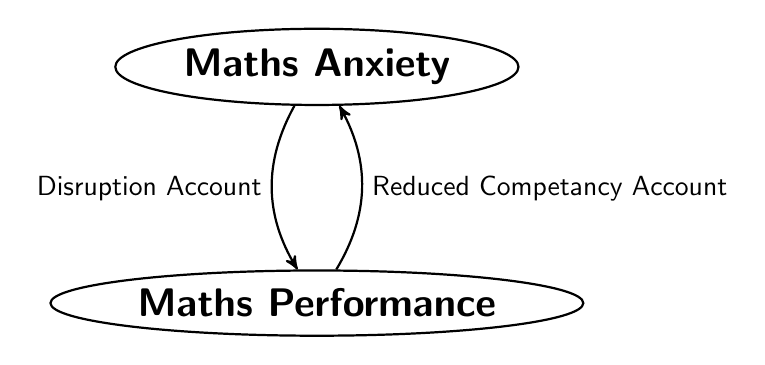
\begin{tikzpicture}[->,>=stealth',auto,node distance=3cm,thick,main node/.style={ellipse,draw,font=\sffamily\Large\bfseries}]
  	\node[main node] (a) {Maths Anxiety};
 	\node[main node] (b) [below of=a] {Maths Performance};

	\path	(a) edge[bend right] node [left] {Disruption Account} (b)
		(b) edge[bend right] node [right] {Reduced Competancy Account} (a);
\end{tikzpicture}
\end{document}
\caption{The Interpretation Account of Ramirez et al. (2018) for the maths anxiety-performance link showing how the Disruption Account and the Reduced Competency Account can be compatible.
\label{fig:ramirez}}
\end{center}
\end{figure}

First, a little more detail on the existing theories. The ``Disruption Account'', spearheaded by the work of Ashcraft et al., is centered around the concept of working memory \cite{Ashcraft2001, Ashcraft2007}. Specifically that anxiety about maths takes up students working memory, which prevents them from using that working memory to complete maths tasks and thereby impacts their performance. The ``Reduced Competency Account'' on the other hand proposes the opposite causality: that lower ability in maths leads to negative experiences associated to maths, which in turn cause maths anxiety to develop. There is also a significant body of work to support this hypothesis, including the milestone meta-analysis of \citeA{Hembree1990} and the longitudinal study of \citeA{Ma2004} which found that although past maths anxiety was correlated with future maths performance it was a small effect, while past maths performance had a strong effect on future maths anxiety.



\subsection*{Complexities in Finding Effective Interventions}

These theoretical views are of course broad oversimplifications of what is an incredibly complex and interconnected topic. They also imply very different approaches for intervention. The ``Reduced Competency Account'' would imply interventions to boost maths performance and hence allow students to experience success in math should also help to reduce maths anxiety. The results of  \citeA{Supekar2015} seem to support this hypothesis as when students are given an intensive 8-week tutoring program to boost their maths skills, this is associated to a reduction in maths anxiety. The earlier work by \citeA{Faust1996} further supports this by demonstrating an anxiety-complexity effect in which low and high maths anxiety groups performed similarly on low complexity problems, but in high complexity problems the high anxiety groups performance was impacted. On the other hand, \citeA{Jansen2013} showed that it is not neccessarily that simple, by showing that when students experience more success they attempt more problems and perform better. However their improved performance is almost completely predicted by the number of problems they attempted, not their experience of success, and their level of maths anxiety was not affected in a significant way which raises a lot of interesting but unanswered questions about this approach. 
	
On the other side of attempted interventions are those in line with the ``Disruption Account'', in which the maths anxiety itself is addressed in the hopes that will free up extra working memory and hence boost students performance.  \citeA{Park2014} demonstrate a direct and successful attempt at this in which they used expressive writing exercises to help guide students self-perceived narratives about their maths experiences and thereby reduce their maths anxiety. Notably the approach of \citeA{Park2014} is in line with successful treatments for clinical anxiety disorders (see \citeA{McNally2007, Becker2007,Foa2005}). Another approach that has shown success in this vein does not attempt to directly reduce the anxiety experienced, but rather reappraise it's symptoms \cite{Jamieson2016}. This is another technique from clinical psychology in which stress is reconceptualised as a coping tool, an evolutionary method for heightening performance in response to a challenge to be overcome, instead of a symptom of exposure to something to be feared and avoided. This change in the perspective of stress is also very much in line with the ``Interpretation Account'' of \citeA{Ramirez2018}.

The work of \citeA{Wang2015} showed the role that intrinsic motivation has mediating the relationship between maths anxiety and performance, and suggested the importance of a mindset centred on viewing the process of learning maths as one of ``productive struggle''. This reconceptualisation to a `productive struggle' model is supported by other literature as well, \citeA{Lin-Siegler2016} exposes students in a classroom to struggles experienced by famous scientists in order to help normalise the concept of productive struggle, and \citeA{Hiebert2007} discuss the importance of this same concept in a maths context.

One of the implications of the ``Interpretation Account'' is that if an intervention targets only one of these two possible links in the cycle (see \reffig{ramirez}), the cycle may re-establish itself after the intervention is over and negate any potential longterm effects. However there is only a very limited amount of research out there on such longterm effects, and several authors have discussed the need for further research into this \cite{Pellicioni2016,Chang2016}. My hypothesis is that a multi-faceted approach targetting both directions simultaneously could disrupt the cycle shown in \reffig{ramirez} and result in significant longterm effects.

\subsection*{Instruments for Measuring Maths Anxiety}

In order to track the effectiveness of these interventions, we will be collating assessment results as a measure of performance, but will also want to measure maths anxiety and maths affect/ self-concept. Significant work has been done over the years to develop psychometrics to measure maths anxiety, almost exclusively consisting of self-reporting surveys (with the exception of some more modern \gls{fmri} work, such as that of \citeA{Lyons2012}). We will use a recently developed scale: the \gls{mas-r} of \citeA{Bai2009}, which has been shown to be remarkably self consistent by incorporating both positive and negative affect items \cite{Bai2011}. It is short, easy to implement, and cheap in comparison to \gls{fmri} methods. In order to measure maths self-concept, \citeA{Jansen2013} modified the Perceived Competence Scale for Children of \citeA{Harter1982} to measure ``Math Competance''. The methodological process imployed by \citeA{Jansen2013} was quite rigorous and so we will use their instrument, or a minor modification thereof (we will do it in English), to measure maths self-concept.












\cleardoublepage
\chapter{Curriculum Mapping}
\label{chap:curriculum}

One of the important roles of university mathematics bridging courses (such as MathsStart and MathsTrack) is to fill the content knowledge gap for students who did not complete mathematics to a sufficiently high level in highschool, or completed it long enough ago that they need to re-learn the material, but wish to commence study at a university level in subjects that have a high level of required knowledge in mathematics. 

There are two angles from which this required knowledge can be seen: the knowledge required for the university study intended, and knowledge expected from highschool graduates. As we will come to see, these two angles or perspectives can be quite dramatically different. From the perspective of knowledge expected from highschool graduates, the \gls{ac} serves as a good guide, but even so the exact content knowledge expected of students having completed highschool in Australia varies for a number of reasons:
\begin{itemize}
	\item To begin with, the \gls{ac} specifies four levels of mathematics: essential mathematics, general mathematics, mathematical methods, and specialist mathematics. Our focus will be on the higher two of these: mathematical methods and specialist mathematics, as these are the ones often associated to university entry into mathematics-intensive courses. 
	\item Different states within Australia teach different curriculums, with varying degrees of alignment to the \gls{ac}. In South Australia the primary curriculum taught in senior secondary school is \gls{sace}, and so we will focus on that.
\end{itemize}
The other perspective is of course the knowledge required for entry level university mathematics courses. This will vary hugely from course to course: a entry level calculus course will require very different knowledge than an entry level statistics course, for example. Even within one discipline of mathematics, different universities will have very different expectations of entry level students: in particular, South Australian universities will often structure their entry level mathematics courses to align with \gls{sace} even though not all their students have completed \gls{sace}, because of the majority who have it is still useful for them to do so. For example, the University of Adeliade re-structured it's first year mathematics courses in 2018 to match changes in \gls{sace}. Similarly, universities interstate will often structure their entry level courses to align with their local senior highschool curriculum. 

This places a difficult tension on mathematics bridging courses as to what content to teach. Although many of the students enrolling in the mathematics bridging courses at the university of adelaide do so with the intention to begin study at the University of Adelaide (and hence might benefit from \gls{sace} structured content), many do not. Even amongst those that do, some may end up going to a different university interstate or even overseas --- plans change. So it is important to try and maintain some connection to a broader set of knowledge expected in general and not neccessarily remain laser focussed on the requirements of the particular university courses most students are going to be attempting. This is one of the reasons why the \gls{ac} is a useful construct as even though some states do not align to the \gls{ac} as well as others, it still forms a guiding structure at a national level and individually considering the curriculum taught in each state is... beyond the scope of this work. Tailoring the content of the bridging courses more narrowly to target entry into particular disciplines (say calculus/ matrix alebra/ statistics for example) could potentially still be of interest down the line, but is likely to be unrealistic with the current resources available to the maths learning center.

This chapter will examine the alignment of the content of MathsStart and MathsTrack (the mathematics bridging courses offered at the university of adelaide) with the \gls{ac} and \gls{sace}. First, in \refsec{content}, some notation will be introduced and the content of each of the three curriculums will be reviewed:
\begin{itemize}
	\item The \gls{ac} senior mathematics subjects mathematical methods and specialist mathematics,
	\item The \gls{sace} curriculum stage 1 mathematics, stage 2 mathematical methods, and stage 2 specialist mathematics,
	\item The University of Adelaide's bridging courses: MathsStart, and MathsTrack.
\end{itemize}
Then, these will be mapped to each other in \refsec{mapping} (see \reffig{mapping}), and alignments/ misalignments discussed. Finally, the discussion throughout around alignment and gaps between the content of these curriculums and courses will be summarised, explanations and reasons for these discrepancies discussed, and potential modifications to content suggested. 

Beyond that, this chapter will also briefly discuss the alignment of these bridging courses to first year university mathematics courses and bridging courses offered by other universities in Australia, and discuss the relationship between the gaps in alignment between the \gls{ac}/\gls{sace} and the bridging courses and the requirements of these first year university courses. 

%However, overall the focus is on the alignment of the bridging courses and \gls{ac}/ \gls{sace}, rather than their alignment to the first year university courses for one clear and important reason: not all students enrolling in these bridging courses are commencing these first year university courses, or may be doing so at a different university in which their first year content is different. Hence, it is most fair to attempt to align the content with the \gls{ac}/\gls{sace} as this is the content other students should be covering in highschool prior to enrolling in university in any case, and hence puts people at a fair standing with those students, and also being aligned with the \gls{ac} in particular is useful for guaranteeing a certain level of knowledge for enrollment in universities interstate. 

\section{Content}
\label{sec:content}

\subsection{Notation}

Each of the senior highschool curriculums, as well as the university bridging courses, being considered here is broken down into topics, with each topic containing a number of key concepts. In \refsec{mapping}, the alignment between these curriculums and bridging courses will be considered thoroughly at both a topic-level, and to the finer detail of particular key concepts. In order to abstract away some of the complexity of considering the topic-level alignment, and be able to present the topic-level alignment in a meaningful way abbreviated codes will be used to identify each topic. These abbreviated codes are presented in \reftab{notation} and will be used for the remainder of this chapter.

\begin{table}[h]
\caption{Abbreviated codes for topics within the \gls{ac} and \gls{sace} senior mathematics subjects: Mathematical Methods nd Specialist Mathematics, as well as the Unviersity of Adelaides bridging courses: MathsStart and MathsTrack. Square brackets ([]) are used to indicate numeric values that can vary. \label{tab:notation}}
\begin{tabular}{ll}
Code & Meaning \\ \hline
 & \\
MMu[\#1]t[\#2] & \gls{ac} Senior Mathematical Methods Unit [\#1], Topic [\#2] \\
MMu[\#1]t[\#2] & \gls{ac} Senior Specialist Mathematics Unit [\#1], Topic [\#2] \\
 & \\
S1M[\#] & \gls{sace} Stage 1 Mathematics, Topic [\#] \\
S2MM[\#] & \gls{sace} Stage 2 Mathematical Methods, Topic [\#] \\
S2SM[\#] & \gls{sace} Stage 2 Specialist Mathematics, Topic [\#] \\
 & \\
MS[\#] & Maths Start, Topic (Booklet) [\#] \\
MT[\#] & Maths Track, Topic (Booklet) [\#]
\end{tabular}
\end{table}

\subsection{Within-Topic Key Concepts}

Description of each topic in the \gls{ac} Mathematical Methods and Specialist Mathematics Topics, \gls{sace} stage 1 mathematics, stage 2 mathematical methods and stage 2 specialist mathematics, and the University of Adelaides MathsStart and MathsTrack programs. For brevity a code is used to identify each topic, see \reftab{notation}, and then for each topic it's name is given in bold followed by a list of the key concepts covered in that topic. These are discussed at length below, and this table is intended to be used as reference material for that discussion.

Some notes on the way the key concepts are summarised:
\begin{itemize}
	\item This key concept summary is intended for a reader deeply familiar with the content, and as such it is heavily condensed and uses notation and terminology without the usually appropriate rigorous definitions. 
	\item Concepts relating to "interpretation" and application in a general sense are ommited. The assumption is that to the intended readers, these should go without saying. For example, in S1M2 the key concept "Quadratic Equations in Vertex and Factorised Form" is included, but this implies a variety of auxillary knowledge which is not explicity included in the key concept summary: the interpretation of roots and vertices, deducing vertices and roots from the equation of a quadratic, or deducing the equation of a quadratic given these bits of information, etc. It is intended that an experienced maths educator should be able to deduce such surrounding concepts from the key concepts that are listed. 
\end{itemize}

Producing this curriculum mapping was a delicate balance between being broad and vague in order to be able to present the entire curriculum mapping within a single frame of view, and yet still be granular enough so that specific content is clear and explicity and useful actionable reccomendations can be made. This balance was acheived by presenting these curriculums are two levels of detail: 
\begin{itemize}
	\item At a topic level (see \reffig{mapping}). This is intended to give the broad strokes, and show the entire mapping in a single frame of view (a page, in this case). It is also intended to be reference material for the following more detailed discussion, to aid the reader in structuring the information contained in the more detialed discussion and place each peice of information into where it belongs in the bigger picture.
	\item At a key concept level, this is what will be presented for the remainder of this section, and intended to be the grandular level at which content is presented specifically enough that reccomended actions can be understood explicitly and implemented easily. Note that although the key concept level is much more granular than the topic level discussion, it is still intended as a summary and does not include every single detail of the content, as discussed above.
\end{itemize}

Note: This is a huge table. I could maybe put it in an apprendix?

% Giant Table of Key Concepts
\documentclass[varwidth=144mm, 12pt]{standalone}

% Multi-page Tables
\usepackage{longtable}

% Math
\usepackage{amsfonts}
\usepackage{amsmath}

% CMU sans serif font.
\usepackage[T1]{fontenc}
\renewcommand*\familydefault{\sfdefault}

\begin{document}
\begin{longtable}{lp{.85\textwidth}}
Code & \textbf{Name} and Key Concepts \\ \hline
& \\ \endhead
%\multicolumn{2}{l}{\gls{ac} Senior Mathematical Methods} \\ 
MMu1t1 & \textbf{Functions and graphs}: Lines, Quadratics, Inverse Proportions, Polynomials, Relations, Translations and Dilations \\
MMu1t2 & \textbf{Trigonometric functions}: Unit Circle, Radians, SOH CAH TOA, Sine Rule, Exact Values, Amplitude/ Period/ Phase, Sum of Angles Identities \\
MMu1t3 & \textbf{Counting and probability}: Binomial Coefficients, Set Complement Intersection and Union, Probability, $P(A\cup{}B) = P(A) + P(B) - P(A\cap{}B)$, Conditional Probability, Independance \\
MMu2t1 & \textbf{Exponential functions}: Index Laws, Fractional Indices, Functions, Asymptotes, Graphs \\
MMu2t2 & \textbf{Arithmetic and geometric sequences and series}: Arithmetic and Geometric Sequences as Recurrence Relations, Limiting Behaviour, and Partial Sum Formulae, Growth and Decay \\
MMu2t3 & \textbf{Introduction to differential calculus} Average Rate of Change, First Principles, Leibniz Notation, Instantaneous Rate of Change, Slope of Tangent, Derivitive of Polynomials, Linearity of Differentiation, Optimisation, Anti-Derivitives, Interpret Position-Time Graphs \\
MMu3t1 & \textbf{Further differentiation and applications}: Define $e$ as $a$ s.t. $\lim_{h \to 0} \frac{a^h - 1}{h} = 1$, Derivitives of $e^x$ $\sin(x)$ and $\cos(x)$, Chain Product and Quotient Rules, Second Derivitives \\
MMu3t2 & \textbf{Integrals}: Integrate Polynomial Exponential and Trigonometric Functions, Linearity of Integration,  Determine Displacement given Velocity, Definite Integrals, Fundamental Theorem of Calculus, (signed) Area Under a Curve \\
MMu3t3 & \textbf{Discrete random variables}: Frequencies, General Properties, Expected Value, Variance, Standard Deviation, Bernoulli and Binomial Distribtions \\
MMu4t1 & \textbf{The logarithmic function}: Logs as Inverse of Exponentials, Log-Scales, Log Function Graphs, Natural Log, $\frac{d}{dx}\ln{x} = \frac{1}{x}$, $\int \frac{1}{x}dx = \ln{x} + c$ for $x > 0$ \\
MMu4t2 & \textbf{Continuous random variables and the normal distribution}: Probability Density Function, Cumulative Distribution Function, Probabilites Expected Value, Variance and Standard Deviation as Integrals, Linear Transformation of Random Variables, Normal Distribution using Technology \\
MMu4t3 & \textbf{Interval estimates for proportions} Simple Random Sampling, Bias, Sample Proportion, Normal Approximation to the Binomial Proportion, Wald Confidence Interval, Trade-Off Between Width and Level of Confidence \\
& \\
%\multicolumn{2}{l}{\gls{ac} Senior Specialist Mathematics} \\ 
SMu1t1 & \textbf{Combinatorics} Multiplication of Possibilities, Factorial Notation, Permutations with and without Repeated Objects, Union of Three Sets, Pigeon-Hole Principle, Combinations, Pascals Triangle \\
SMu1t2 & \textbf{Vectors in the plane}: Magnetude and Direction, Scalar Multiplication, Addition and Substraction as a Triangle, Vector Notation, $a\textbf{i} + b\textbf{j}$ Notation, Scalar Dot Product, Projection, Parallel and Perpendicular Vectors \\
SMu1t3 & \textbf{Geometry}: Notation for Implication ($\Rightarrow$) and Equivalence ($\Leftrightarrow$), Converse ($B \Rightarrow A$) Negation ($\neg A \Rightarrow \neg B$) and Contrapositive ($\neg B \Rightarrow \neg A$), Proof by Contradiction, $\forall$ and $\exists$ Notation, Counter-Examples, Circle Theorems, Quadrilateral Proofs in $\mathbb{R}^2$ \\
SMu2t1 & \textbf{Trigonometry}: Graph and Solve Trig Functions, Prove Various Trig Indentities, Reciprocal Trig Functions \\
SMu2t2 & \textbf{Matrices}: Notation, Addition and Scalar Multiplication of Matrices, Multiplicative Identity and Inverse, Determinant, Matrices as Transformations \\
SMu2t3 & \textbf{Real and complex numbers}: Rationality and Irrationality, Induction, $i = \sqrt{-1}$, Complex Numbers $a + bi$ and Arithmetic ($+$, $-$, $\times$, $\div$), Complex Conjugates, Complex Plane,  Complex Conjugate Roots of Polynomials \\
SMu3t1 & \textbf{Complex numbers}: Modulus and Argument, Arithmetic ($\times$, $\div$, and $z^n$) in Polar Form, Convert between Polar and Cartesian Form, De Moivre's Theorem, Roots of Complex Numbers, Factorising Polynomials \\
SMu3t2 & \textbf{Functions and sketching graphs}: Composition of Functions, One-to-One, Inverse Functions, Absolute Value Function, Rational Functions \\
SMu3t3 & \textbf{Vectors in three dimensions}: $a\textbf{i} + b\textbf{j} + c\textbf{k}$ Notation, Equation for Spheres, Parameterised Vector Equations, Equations of Lines, the Cross Product, Equation for a Plane, Systems of Linear Equation (Elimination Method) and Geometric Interpretation of Solutions, Kinematics via Differentiation of Vector Equations, Projectile and Circular Motion \\
SMu4t1 & \textbf{Integration and applications of integration} Substitution, $\int \frac{1}{x}dx = \ln{|x|} + c$ for $x \neq 0$, Inverse Trig Functions and their Derivitives, Integrate $\frac{\pm1}{\sqrt{a^2-x^2}}$ and $\frac{a}{a^2 + x^2}$, Partial Fractions, Integration by Parts, Volume of Solids of Revolution, Numerical Integration using Technology \\
SMu4t2 & \textbf{Rates of change and differential equations}: Implicit Differentiation, First-Order Seperable Differential Equations, The Logistic Equation, Kinematics (Rates of Change) \\
SMu4t3 & \textbf{Statistical inference}: Central Limit Theorem and the Resulting Confidence Interval for a Mean \\
& \\
%\multicolumn{2}{l}{\gls{sace} Stage 1 Mathematics} \\ 
S1M1 & \textbf{Functions and graphs}: Equations for a Line, Slope, y-intercept, Intersection of Lines, Reciprocal Function, Asymptotes, Functions vs Relations, Domain, Range, Function Notation \\
S1M2 & \textbf{Polynomials}: Quadratic Equations in Vertex and Factorised Forms, Quadratic Formula, Completing the Square, The Leading Coefficient and Degree of a Polynomials, Cubics, Quartics\\
S1M3 & \textbf{Trigonometry}: Pythagoras, SOH CAH TOA, Cosine Rule, Sine Rule, Unit Circle, Sine and Cosine Functions, Radians, Length of Arc, Area of Sector, Amplitude, Period, Phase, $\tan{x} = \frac{\sin{x}}{\cos{x}}$ \\
S1M4 & \textbf{Counting and statistics}: Factorial, Permutations, Multiplication Principle, Combinations, Discrete vs Continuous Random Variables, Mean, Median, Mode, Range, Interquartile Range, Standard Deviation, Normal Distribution, \\
S1M5 & \textbf{Growth and decay}: Index and Logarithm Laws, Exponential Functions and their Graphs \\
S1M6 & \textbf{Introduction to differential calculus}: Average Rate of Change, First Principles, Notation $f'(x) = \frac{df}{dx}$, $\frac{d}{dx}x^n = nx^{n-1}$, Linearity of Differentiation, Slope of Tangent, Increasing vs Decreasing, Local and Global Maxima and Minima, Stationary Points, Sign Diagram \\
S1M7 & \textbf{Arithmetic and geometric sequences and series}: \\
S1M8 & \textbf{Geometry}: \\
S1M9 & \textbf{Vectors in the plane}: \\
S1M10 & \textbf{Further Trigonometry}: \\
S1M11 & \textbf{Matrices}: \\
S1M12 & \textbf{Real and complex numbers}: \\
& \\
%\multicolumn{2}{l}{\gls{sace} Stage 2 Mathematical Methods} \\ 
S1MM1 & \textbf{Further differentiation and applications}: \\
S1MM2 & \textbf{Discrete random variables}: \\
S1MM3 & \textbf{Integral calculus}: \\
S1MM4 & \textbf{Logarithmic functions}: \\
S1MM5 & \textbf{Continuous random variables and the normal distribution}: \\
S1MM6 & \textbf{Sampling and confidence intervals}: \\
& \\
%\multicolumn{2}{l}{\gls{sace} Stage 2 Specialist Mathematics} \\ 
S1SM1 & \textbf{Mathematical induction}: \\
S1SM2 & \textbf{Complex numbers}: \\
S1SM3 & \textbf{Functions and sketching graphs}: \\
S1SM4 & \textbf{Vectors in three dimensions}: \\
S1SM5 & \textbf{Integration techniques and applications}: \\
S1SM6 & \textbf{Rates of change and differential equations}: \\
& \\
%\multicolumn{2}{l}{UofA MathStart} \\ 
MS1 & \textbf{Numbers \& Functions}: \\
MS2 & \textbf{Linear Functions}: \\
MS3 & \textbf{Quadratic Functions}: \\
MS4 & \textbf{Rational Functions}: \\
MS5 & \textbf{Trigonometry I}: \\
MS6 & \textbf{Trigonometry II}: \\
MS7 & \textbf{Exponential Functions}: \\
MS8 & \textbf{Logarithms}: \\
& \\
%\multicolumn{2}{l}{UofA MathTrack} \\ 
MT1 & \textbf{Polynomials}: \\
MT2 & \textbf{Matrices}: \\
MT3 & \textbf{Vectors and Applications}: \\
MT4 & \textbf{Systems of Linear Equations}: \\
MT6 & \textbf{Differentiation}: \\
MT7 & \textbf{Applications of Differentiation}: \\
MT8 & \textbf{Exponential and Logarithm Functions}: \\
MT9 & \textbf{Integration}: \\
\end{longtable}
\end{document}


\subsection{\gls{ac} Mathematical Methods and Specialist Mathematics}

 \gls{ac} has four levels of mathmatics, including also essential and general mathematics. Mathematical Methods and Specialist Mathematics are the two highest level mathematics, intended (partly) for preparation to university entry. Broadly speaking, the content of these two subjects can be grouped into several areas:
\begin{itemize}
	\item Functions and Graphs, which is broken up primarily into families of functions, with some extra concepts thown into some generalist topics:
		\begin{itemize}	
			\item Polynomials and Rational Functions (MMu1t1, SMu3t2),
			\item Exponentials and Logarithms (MMu2t1, MMu2t2, MMu4t1)
			\item Trigonometric Functions (MMu1t2, SMu2t1)
		\end{itemize}
	\item Calculus, which is largely structured similarly to the Functions and Graphs: breaking it up by the type of function you are doing calculus on, splitting up differentiation from integration, and throwing in rules of differentiation and approaches to integration with a few extra concepts along the way (MMu2t3, MMu3t1, MMu3t2, SMu4t1, SM4t2).
	\item Geometry and Linear Algebra: Mostly vectors, with some matrices, systems of equations, and even circle theorems. This is the topic in which the concept of proof is primarily attempted to be introduced, and perhaps that is the reason why it is entirely contained within the Specialist Mathematics curriculum (SMu1t2, SMu1t3, SMu2t2, SMu3t3),
	\item Complex Numbers, as well as rational/ irrational numbers, etc. (SMu2t3, SMu3t1), and finally
	\item Probability and Statistics, with some combinatorics thrown in for good measure (MMu1t3, MMu3t3, MMu4t2, MMu4t3, SMu1t1, SMu4t3)
\end{itemize}
Although there are a couple of topics (MMu2t2 for example) which although they relate to these broader areas, also contain a substantial amount of other content.

More detailed discussion of the specific key concepts of interest will follow in \refsec{mapping} as a natural part of comparisons between curriculums, as that is where the specifics will be important. These sections are intended to give a broader overview of the structure of the content in these curriculums

\subsection{\gls{sace} Stage 1 Mathematics, Stage 2 Mathematical Methods and Specialist Mathematics}

\gls{sace} follows the \gls{ac} fairly well at a broad level (although there are differences in the details, which will be discussed in \refsec{mapping}. Broadly though the topics in the three \gls{sace} subjects here, although split into three subjects instead of two, can be broadly grouped into areas much the same as the \gls{ac}:
\begin{itemize}
	\item Functions and Graphs, which is broken roughy as:
		\begin{itemize}	
			\item General Concepts (S1M1, S2SM3),
			\item Polynomials and Rational Functions (S1M2, S2SM3),
			\item Exponentials and Logarithms (S1M5, S2MM4, S1M7)
			\item Trigonometric Functions (S1M3, S1M10)
		\end{itemize}
	\item Calculus, which similarly split up by the type of function you are doing calculus on, differentiation vs integration, and throwing in rules of differentiation and approaches to integration with a few extra concepts along the way (S1M6, S2MM1, S2MM3, S2MM4, S2SM5, S2SM6).
	\item Geometry and Linear Algebra: Mostly vectors, with some matrices, systems of equations, and even circle theorems. This is the topic in which the concept of proof is primarily attempted to be introduced, and perhaps that is the reason why it is entirely contained within the Specialist Mathematics curriculum (S1M8, S1M9, S1M11, S2SM4),
	\item Complex Numbers, as well as rational/ irrational numbers, etc. (S1M12, S2SM2), and finally
	\item Probability and Statistics, with some combinatorics thrown in for good measure is included almost exclusively in Stage 2 Mathematical Methods (S1M4, S2MM2, S2MM5, S2MM6)
\end{itemize}
Although there are a couple of topics (S1M7,for example --- very similarly to MMu2t2) which although they relate to these broader areas, also contain a substantial amount of other content. This grouping also leaves one topic out in the \gls{sace} context: S2SM1 which is essentially just the concept of mathematical induction.



\subsection{MathsStart and MathsTrack}

MathsStart can be seen as essentially an introduction to functions, MathsTrack then takes this, and extends it primarily to calculus, taking a little detour along the way to cover some vector and matrix geometry/ systems of linear equations concepts. So broadly grouping the topics in a way analogous to above:
\begin{itemize}
	\item Functions and Graphs, roughly broken up into:
		\begin{itemize}
			\item General Concepts (MS1, MS2),
			\item Polynomials and Rational Functions (MS3, MS4, MT1),
			\item Exponentials and Logarithms (MS7, MS8), and 
			\item Trigonometry (MS5, MS6)
		\end{itemize}
	\item Calculus, similarly first introducing differentiation on polynomials with various other general concepts (MT6, MT7) and then exponentials and logarithms (MT8) and finally also integration (MT9).
	\item Geometry and Linear Algebra (MT2, MT3, MT4).
\end{itemize}

Note the missing topic 5 in MathsTrack, this used to be part of the course some time ago but is currently no longer included in the content of the course, and so is not included here.








\section{Curriculum Mapping}
\label{sec:mapping}

\reffig{mapping} shows the topic-level alignment between the \gls{ac} (senior mathematical methods and specialist mathematics), \gls{sace} (stage 1 mathematics, stage 2 mathematical methods and stage 2 specialist mathematics), MathsStart and MathsTrack. This is the broad, eagle-eye, view of the alignment between the content in these topics.

Although key concept level alignment between topics connected with lines in \reffig{mapping} is not always perfect, it is fairly strong in most cases. Individual cases with any misalignment will be discussed in the remainder of this chapter.

\begin{figure}[p]
\begin{center}
% TiKz
\documentclass[tikz, 12pt]{standalone}
\usetikzlibrary{positioning}
\usetikzlibrary{shapes}

% Math
\usepackage{amsfonts}
\usepackage{amsmath}

% CMU sans serif font.
\usepackage[T1]{fontenc}
\renewcommand*\familydefault{\sfdefault}

\begin{document}
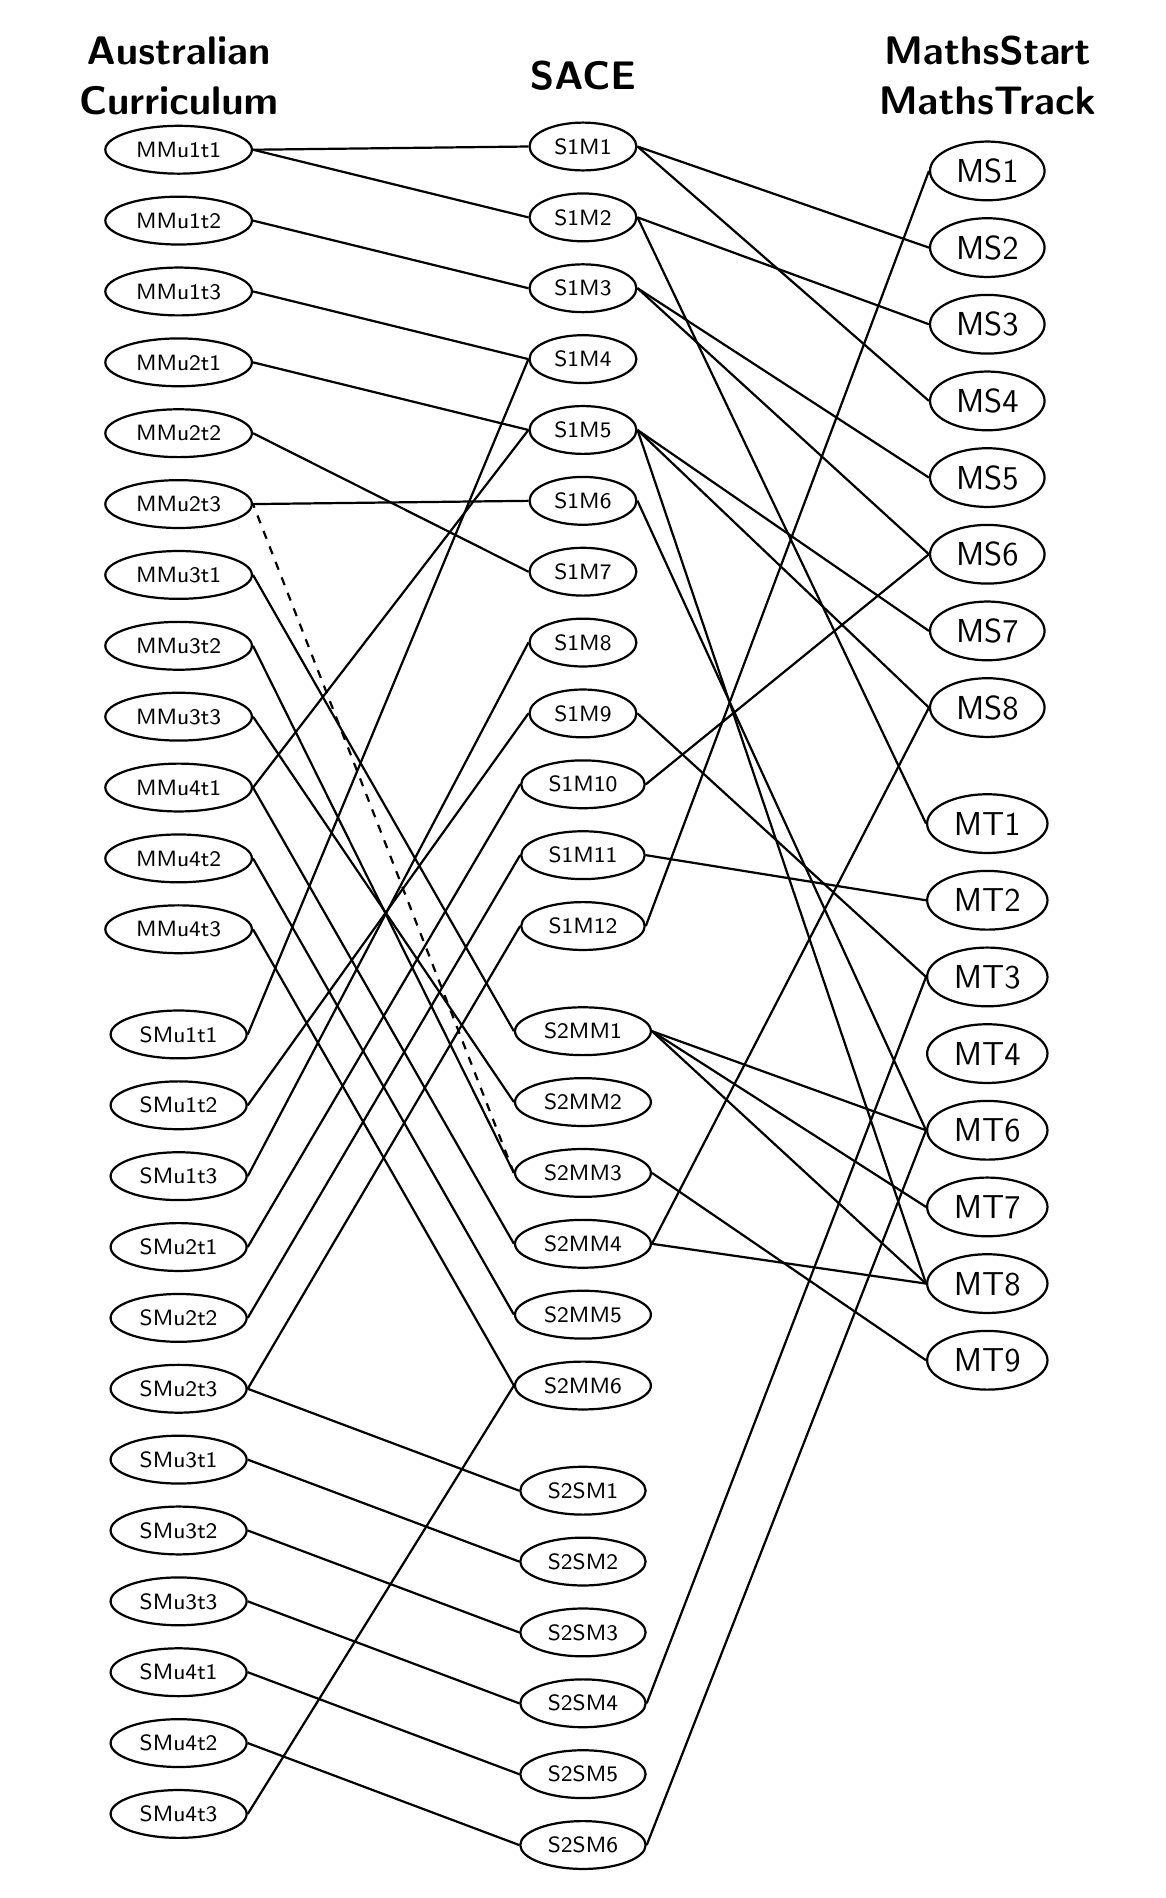
\begin{tikzpicture}[node distance=0.9cm,thick,topic node/.style={ellipse,draw,font=\footnotesize},unit node/.style={ellipse,draw,font=\large}]

	% MathsStart
	\node[font=\Large\bfseries, text width = 3.6cm, align=center] (ms) {MathsStart MathsTrack};
  	\node[unit node] (ms1) [below=0.2cm of ms] {MS1};
  	\node[unit node] (ms2) [below=0.2cm of ms1] {MS2};
  	\node[unit node] (ms3) [below=0.2cm of ms2] {MS3};
  	\node[unit node] (ms4) [below=0.2cm of ms3] {MS4};
  	\node[unit node] (ms5) [below=0.2cm of ms4] {MS5};
  	\node[unit node] (ms6) [below=0.2cm of ms5] {MS6};
  	\node[unit node] (ms7) [below=0.2cm of ms6] {MS7};
  	\node[unit node] (ms8) [below=0.2cm of ms7] {MS8};
%  	\node[unit node] (ms1) [below=0.2cm of ms] {Functions};
%  	\node[unit node] (ms2) [below=0.2cm of ms1] {Linear};
%  	\node[unit node] (ms3) [below=0.2cm of ms2] {Quadratic};
%  	\node[unit node] (ms4) [below=0.2cm of ms3] {Rational};
%  	\node[unit node] (ms5) [below=0.2cm of ms4] {Trigonometry I};
%  	\node[unit node] (ms6) [below=0.2cm of ms5] {Trigonometry II};
%  	\node[unit node] (ms7) [below=0.2cm of ms6] {Exponential};
%  	\node[unit node] (ms8) [below=0.2cm of ms7] {Logarithm};

	% MathsTrack
  	\node[unit node] (mt1) [below=0.7cm of ms8] {MT1};
  	\node[unit node] (mt2) [below=0.2cm of mt1] {MT2};
  	\node[unit node] (mt3) [below=0.2cm of mt2] {MT3};
  	\node[unit node] (mt4) [below=0.2cm of mt3] {MT4};
  	\node[unit node] (mt6) [below=0.2cm of mt4] {MT6};
  	\node[unit node] (mt7) [below=0.2cm of mt6] {MT7};
  	\node[unit node] (mt8) [below=0.2cm of mt7] {MT8};
  	\node[unit node] (mt9) [below=0.2cm of mt8] {MT9};
%  	\node[unit node] (mt1) [below=0.8cm of ms8] {Polynomials};
%  	\node[unit node] (mt2) [below=0.2cm of mt1] {Matrices};
%  	\node[unit node] (mt3) [below=0.2cm of mt2] {Vectors};
%  	\node[unit node] (mt4) [below=0.2cm of mt3] {Systems of Eqns};
%  	\node[unit node] (mt6) [below=0.2cm of mt4] {Differentiation};
%  	\node[unit node] (mt7) [below=0.2cm of mt6] {Differentiation Apps};
%  	\node[unit node] (mt8) [below=0.2cm of mt7] {Exp and Log};
%  	\node[unit node] (mt9) [below=0.2cm of mt8] {Integration};
  	
	% SACE
	\node[font=\Large\bfseries] (sace) [left=2.4cm of ms] {SACE};
  	\node[topic node] (ss1m1) [below of=sace] {S1M1};
  	\node[topic node] (ss1m2) [below of=ss1m1] {S1M2};
  	\node[topic node] (ss1m3) [below of=ss1m2] {S1M3};
  	\node[topic node] (ss1m4) [below of=ss1m3] {S1M4};
  	\node[topic node] (ss1m5) [below of=ss1m4] {S1M5};
  	\node[topic node] (ss1m6) [below of=ss1m5] {S1M6};
  	\node[topic node] (ss1m7) [below of=ss1m6] {S1M7};
  	\node[topic node] (ss1m8) [below of=ss1m7] {S1M8};
  	\node[topic node] (ss1m9) [below of=ss1m8] {S1M9};
  	\node[topic node] (ss1m10) [below of=ss1m9] {S1M10};
  	\node[topic node] (ss1m11) [below of=ss1m10] {S1M11};
  	\node[topic node] (ss1m12) [below of=ss1m11] {S1M12};
%  	\node[topic node] (ss1m1) [below of=sace] {Functions I};
%  	\node[topic node] (ss1m2) [below of=ss1m1] {Polynomials};
%  	\node[topic node] (ss1m3) [below of=ss1m2] {Trigonometry I};
%  	\node[topic node] (ss1m4) [below of=ss1m3] {Combinatorics};
%  	\node[topic node] (ss1m5) [below of=ss1m4] {Exponentials};
%  	\node[topic node] (ss1m6) [below of=ss1m5] {Differentiation I};
%  	\node[topic node] (ss1m7) [below of=ss1m6] {Sequences};
%  	\node[topic node] (ss1m8) [below of=ss1m7] {Circle Theorems};
%  	\node[topic node] (ss1m9) [below of=ss1m8] {Vectors ($\mathbb{R}^2$)};
%  	\node[topic node] (ss1m10) [below of=ss1m9] {Trigonometry II};
%  	\node[topic node] (ss1m11) [below of=ss1m10] {Matrices};
%  	\node[topic node] (ss1m12) [below of=ss1m11] {Complex ($\mathbb{C}$) I};
  	
  	\node[topic node] (ss2mm1) [below=0.7cm of ss1m12] {S2MM1};
  	\node[topic node] (ss2mm2) [below of=ss2mm1] {S2MM2};
  	\node[topic node] (ss2mm3) [below of=ss2mm2] {S2MM3};
  	\node[topic node] (ss2mm4) [below of=ss2mm3] {S2MM4};
  	\node[topic node] (ss2mm5) [below of=ss2mm4] {S2MM5};
  	\node[topic node] (ss2mm6) [below of=ss2mm5] {S2MM6};
%  	\node[topic node] (ss2mm1) [below=1cm of ss1m12] {Differentiation II};
%  	\node[topic node] (ss2mm2) [below of=ss2mm1] {Discrete RV};
%  	\node[topic node] (ss2mm3) [below of=ss2mm2] {Integration I};
%  	\node[topic node] (ss2mm4) [below of=ss2mm3] {Logarithms};
%  	\node[topic node] (ss2mm5) [below of=ss2mm4] {Continuous RV};
%  	\node[topic node] (ss2mm6) [below of=ss2mm5] {Sampling};
  	
  	\node[topic node] (ss2sm1) [below=0.7cm of ss2mm6] {S2SM1};
  	\node[topic node] (ss2sm2) [below of=ss2sm1] {S2SM2};
  	\node[topic node] (ss2sm3) [below of=ss2sm2] {S2SM3};
  	\node[topic node] (ss2sm4) [below of=ss2sm3] {S2SM4};
  	\node[topic node] (ss2sm5) [below of=ss2sm4] {S2SM5};
  	\node[topic node] (ss2sm6) [below of=ss2sm5] {S2SM6};  	
%  	\node[topic node] (ss2sm1) [below=1cm of ss2mm6] {Induction};
%  	\node[topic node] (ss2sm2) [below of=ss2sm1] {Complex ($\mathbb{C}$) II};
%  	\node[topic node] (ss2sm3) [below of=ss2sm2] {Functions II};
%  	\node[topic node] (ss2sm4) [below of=ss2sm3] {Vectors ($\mathbb{R}^3$)};
%  	\node[topic node] (ss2sm5) [below of=ss2sm4] {Integration II};
%  	\node[topic node] (ss2sm6) [below of=ss2sm5] {DEs};  	
  	
	% Australian Curriculum
	\node[font=\Large\bfseries, text width = 3.6cm, align=center] (ac) [left=2.4cm of sace] {Australian Curriculum};
  	\node[topic node] (acmmmu1t1) [below=0cm of ac] {MMu1t1};
  	\node[topic node] (acmmmu1t2) [below of=acmmmu1t1] {MMu1t2};
  	\node[topic node] (acmmmu1t3) [below of=acmmmu1t2] {MMu1t3};
  	\node[topic node] (acmmmu2t1) [below of=acmmmu1t3] {MMu2t1};
  	\node[topic node] (acmmmu2t2) [below of=acmmmu2t1] {MMu2t2};
  	\node[topic node] (acmmmu2t3) [below of=acmmmu2t2] {MMu2t3};
  	\node[topic node] (acmmmu3t1) [below of=acmmmu2t3] {MMu3t1};
  	\node[topic node] (acmmmu3t2) [below of=acmmmu3t1] {MMu3t2};
  	\node[topic node] (acmmmu3t3) [below of=acmmmu3t2] {MMu3t3};
  	\node[topic node] (acmmmu4t1) [below of=acmmmu3t3] {MMu4t1};
  	\node[topic node] (acmmmu4t2) [below of=acmmmu4t1] {MMu4t2};
  	\node[topic node] (acmmmu4t3) [below of=acmmmu4t2] {MMu4t3};
  	
  	\node[topic node] (acmsmu1t1) [below=0.7cm of acmmmu4t3] {SMu1t1};
  	\node[topic node] (acmsmu1t2) [below of=acmsmu1t1] {SMu1t2};
  	\node[topic node] (acmsmu1t3) [below of=acmsmu1t2] {SMu1t3};
  	\node[topic node] (acmsmu2t1) [below of=acmsmu1t3] {SMu2t1};
  	\node[topic node] (acmsmu2t2) [below of=acmsmu2t1] {SMu2t2};
  	\node[topic node] (acmsmu2t3) [below of=acmsmu2t2] {SMu2t3};
  	\node[topic node] (acmsmu3t1) [below of=acmsmu2t3] {SMu3t1};
  	\node[topic node] (acmsmu3t2) [below of=acmsmu3t1] {SMu3t2};
  	\node[topic node] (acmsmu3t3) [below of=acmsmu3t2] {SMu3t3};
  	\node[topic node] (acmsmu4t1) [below of=acmsmu3t3] {SMu4t1};
  	\node[topic node] (acmsmu4t2) [below of=acmsmu4t1] {SMu4t2};
  	\node[topic node] (acmsmu4t3) [below of=acmsmu4t2] {SMu4t3};

	% Australian Curriculum -- SACE links
	\draw (ss1m1.west) -- (acmmmu1t1.east);
	\draw (ss1m2.west) -- (acmmmu1t1.east);
	\draw (ss1m3.west) -- (acmmmu1t2.east);
	\draw (ss1m4.west) -- (acmmmu1t3.east);
	\draw (ss1m4.west) -- (acmsmu1t1.east);
	\draw (ss1m5.west) -- (acmmmu2t1.east);
	\draw (ss1m5.west) -- (acmmmu4t1.east);
	\draw (ss1m6.west) -- (acmmmu2t3.east);
	\draw (ss1m7.west) -- (acmmmu2t2.east);
	\draw (ss1m8.west) -- (acmsmu1t3.east);
	\draw (ss1m9.west) -- (acmsmu1t2.east);
	\draw (ss1m10.west) -- (acmsmu2t1.east);
	\draw (ss1m11.west) -- (acmsmu2t2.east);
	\draw (ss1m12.west) -- (acmsmu2t3.east);
		
	\draw (ss2mm1.west) -- (acmmmu3t1.east);
	\draw (ss2mm2.west) -- (acmmmu3t3.east);
	\draw (ss2mm3.west) -- (acmmmu3t2.east);
	\draw[dashed] (ss2mm3.west) -- (acmmmu2t3.east);
	\draw (ss2mm4.west) -- (acmmmu4t1.east);
	\draw (ss2mm5.west) -- (acmmmu4t2.east);
	\draw (ss2mm6.west) -- (acmmmu4t3.east);
	\draw (ss2mm6.west) -- (acmsmu4t3.east);

	\draw (ss2sm1.west) -- (acmsmu2t3.east);
	\draw (ss2sm2.west) -- (acmsmu3t1.east);
	\draw (ss2sm3.west) -- (acmsmu3t2.east);
	\draw (ss2sm4.west) -- (acmsmu3t3.east);
	\draw (ss2sm5.west) -- (acmsmu4t1.east);
	\draw (ss2sm6.west) -- (acmsmu4t2.east);

	% MathsTrack to SACE links
	\draw (mt1.west) -- (ss1m2.east);
	\draw (mt2.west) -- (ss1m11.east);
	\draw (mt3.west) -- (ss1m9.east);
	\draw (mt3.west) -- (ss2sm4.east);
	\draw (mt6.west) -- (ss1m6.east);
	\draw (mt6.west) -- (ss2mm1.east);
	\draw (mt6.west) -- (ss2sm6.east);
	\draw (mt7.west) -- (ss2mm1.east);
	\draw (mt8.west) -- (ss1m5.east);
	\draw (mt8.west) -- (ss2mm1.east);
	\draw (mt8.west) -- (ss2mm4.east);
	\draw (mt9.west) -- (ss2mm3.east);

	% MathsStart to SACE links
	\draw (ms1.west) -- (ss1m12.east);
	\draw (ms2.west) -- (ss1m1.east);
	\draw (ms3.west) -- (ss1m2.east);
	\draw (ms4.west) -- (ss1m1.east);
	\draw (ms5.west) -- (ss1m3.east);
	\draw (ms6.west) -- (ss1m3.east);
	\draw (ms6.west) -- (ss1m10.east);
	\draw (ms7.west) -- (ss1m5.east);
	\draw (ms8.west) -- (ss1m5.east);
	\draw (ms8.west) -- (ss2mm4.east);
	

  	
\end{tikzpicture}
\end{document}
\caption{Curriculum Mapping\label{fig:mapping}}
\end{center}
\end{figure}

\subsection{\gls{ac} to \gls{sace}}

At a glance, there appears to be a very good one-to-one alignment at the topic level between the \gls{ac} and \gls{sace}. Broadly speaking the biggest difference between these two curriculums is their structure. The \gls{ac} content is structured into two subjects (mathematical methods and specialist mathematics) which span "senior highschool", which most commonly would equate to both years 11 and 12 in Australia. Each of these two subjects contains 12 topics. The \gls{sace} content on the other hand is split into stage 1 (commonly year 11 in Australia) and stage 2 (commonly year 12), stage 1 consists of a single subject "mathematics" with 12 topics, and stage 2 is split into two (mathematical methods and specialist mathematics) each with 6 topics. So the total number of topics is actually the same accross the board between the \gls{ac} and \gls{sace}, and they seem to match almost exactly with a pattern in which the first 6 topics of both the \gls{ac} mathematical methods and speciaist mathematics constitute \gls{sace} stage 1 mathematics and the remaining 6 topics in each of the \gls{ac} subjects align to the corresponding \gls{sace} stage 2 subject.

Note: The content is almost identical between these, the structure is simply different. Given how we don't really care about the structure, but rather care about the content maybe it would be more useful to structure this discussion into content areas rather than base it on the curriculum structure.


As usual however, the devil is in the details:
\begin{itemize}
	\item In terms of Functions and Graphs:
		\begin{itemize}
			\item Gerneral Concepts, Polynomials and Rational Functions: In both the \gls{ac} and \gls{sace} this area is split into two: basic introduction and advanced concepts.The basic introduction topics align well (MMu1t1 to S1M1 and S1M2), with only slight differences in terminology (\gls{ac} refers to inverse proportion while \gls{sace} refers to reciprocal for example) and focus (\gls{sace} puts much more of an emphasis on polynomials, seperating it into it's own topic (S1M2) and breaking it down into much more granular concepts). The advanced concepts are covered in SMu3t2 and S2SM3 are essentially identical.
			\item Exponentials and Logarithims: There is essentially perfect alignment between the concepts for logarithms between MMu4t1 and S2MM4. Concepts around exponentials however are a little less straightforward. Similarly, MMu2t2 is almost exactly the same as S1M7, they are both centered on the introduction of recurrance relations, partial sums, and linking this back to exponential functions. I include these topics under exponentials as they link to those concepts, but really they focus on concepts around sequences and series, it's just they don't connect to anything else better than they connect with exponentials, so here they go, really they are a fairly distinct set of concepts though. However it is in the alignment between MMu2t1 and S15 that there is a difference: S15 includes Log-Laws, while MM2t1 does not, focusing only on Index Laws. This is not actually a difference in content between the \gls{ac} and \gls{sace} as the log laws are covered in the \gls{ac} in MMu4t1. They are actually repeated in the \gls{sace} curriculum, covered both in S1M5 and then again in S2MM4.
			\item Trigonometry: MMu1t2 matches almost identically to S1M3, with the biggest difference being that in the \gls{ac} the unit circle interpretations/ definitions of $\sin(x)$, $\cos(x)$, and in particular $\tan(x)$ are emphasised, where in \gls{sace} $\tan(x)$ in particular is introduced instead as $\frac{\sin(x)}{\cos(x)}$. That being the biggest difference between the two should emphasise how similar they are in terms of content. Similarly, SMu2t1 and S1M10 align just about perfectly. 
		\end{itemize}
	\item Calculus: 
		\begin{itemize}
			\item SMu4t1 aligns perfectly with S2SM5, both covering integration by parts, by substitution, inverse trig substitutions in integration problems, volume of solids of revolution, partial fractions and area between two curves. 
			\item SMu4t2 aligns well to S2SM6, both covering implicit differentiation, solving first-order seperable differential equations, and the logistic equation. However there are some differences in that the \gls{ac} goes on to focus on rates of change, while \gls{sace} instead decides to focus on parameterised curves, trigonometric parameterisations, etc.
			\item MMu2t3 and S1M6 both introduce differentiation by leading in with the concept of average rate of change, first principles and lead into linearity of differentiation, derivitives of polynomials, slope of the tangent and optimisation but in \gls{sace} S1M6 introduces the terms ``increasing'' and ``decreasing'' and sign diagrams, which are not mentioned in MMu2t3 (or \gls{ac}?), while MMu2t3 introduces the concept of an antiderivative.  
			\item MMu3t1 and S2MM1 align perfectly introducing the chain, product, and quotient rule. Introducing $e = 2.718\hdots$ in the same way (using first principles to explore $\frac{d}{dx}{a^x}$ for different $a$, derivitives of $\sin(x)$ and $\cos(x)$, and second derivatives.  
			\item MMu3t2 and S2MM3 are very closely aligned, both introducing both definite and indefinite integrals of polynomials, exponentials, and trigonometric functions, linearity of integration and the fundamental theorem of calculus, they have diverge slightly in their approach to definite integrals. In particular, \gls{sace} S2MM3 introduces the concepts of upper and lower sums and the definite integral as the unique number between the two as the size of the rectangles approaches zero, while in the \gls{ac} MMu3t2 this is not discussed. Also, S2MM3 introduces anti-differentiation, a concept introduced in the \gls{ac} MMu2t3 but not introduced in \gls{sace} S1M6, instead being covered here in S2MM3.
		\end{itemize}
	Note how although most derivatives are introduced in differentiation specific topics, $\frac{d}{dx}\ln(x)$ is introduced in a seperate topic entirely about logarithm functions in both the \gls{ac} (MMu4t1) and \gls{sace} (S2MM4), and I categorise these topics under `Functions and Graphs' above because I see these topics as an introduction to logarithms, but they do also contain concepts around calculus (of logarithm functions).
	\item Geometry and Linear Algebra
		\begin{itemize}
			\item Vectors in the Plane are covered in SMu1t2 and S1M9, with the content being very well aligned and the only really notable difference being the inclusion of geometric vector proofs in \gls{sace} S1M9 which is not included in SMu1t2, instead being introduced but restricted to other topics... i.e.
			\item Proof and Circle Theorems which are covered in SMu1t3 to S1M8. Both these cover the same "content" in the sense of theorems: circle theorems, but they also both attempt to broach the difficult topic of proof, methods of proof, and some of the language around proof, and they take quite different approaches to this. The \gls{ac} SMu1t2 is quite explicit specifing the introduction of language around formal logic: imlication, equivalence, converse, negative, contrapositive, contradiction, 'for all' and 'there exists', counter-examples. On the other hand, \gls{sace} S1M8 simply specifies proof to be investigated as "justification of properties of circles", and only breifly mentions specifics of language and methods as suggestions not specificying them as being required components of the curriculum and instead leaving the approach and specific content chosen to be used to introduce the concept of proof much more open to interpretation by the teacher.
			\item Matrices, covered in SMu2t2 and S1M11 are essentially identical in content covering matrix notation, linear combinations of matrices, matrix multiplication, matrix indentity and inverses (and determinants), and the perspective of matrices as linear transformations. 
			\item Vectors in 3D in SMu3t3 and S2SM4 are also introduced very similarly in terms of content: cross product, equations for lines and planes, systems of equations and geometric interpretation of their solutions.  One of the main differences however is in how they apply these concepts, the \gls{ac} SMu3t3 includes a focus on parameterised vector equations, the equation for a sphere, and in particular kinematics: projectile and circular motion in 3D, which are not coverted in \gls{sace} S2SM4, which instead remains more abstract with these concepts, and on the other hand the examples required are less complex to interpret. 
		\end{itemize}
	\item Complex Numbers are introduced in two topics, a basic an advanced topic, in both curriculums. The basic topics, SMu2t3 in the \gls{ac} and S1M12 in \gls{sace} are quite similar in their base content: rational/ irrational numbers, $i$, complex arithmetic, conjugates, and complex roots of polynomials. However there are a couple of key differences between the two: first, induction is introduced in the \gls{ac} SMu2t3 while in \gls{sace} it is seperated into it's own seperate topic: S2SM1. The second key difference is that interval notation is explicitly introduced in \gls{sace} S1M12, while in the \gls{ac} interval notation seems to be neglected. The advanced topics SMu3t1 and S2SM2 on the other hand align almost perfectly in content.
	\item Probability and Statistics is the topic area in which the alignment between the \gls{ac} and \gls{sace} is at it's loosest, and the most substantial differences in content exist between the two.  
		\begin{itemize}
			\item Combinatorics: MMu1t3, SMu1t1, and S1M4. The overlap between the \gls{ac} and \gls{sace} for these topics is essentially concepts around permutations, factorial (and the `multiplication principle'), combinations. Although it is notable that the \gls{ac} MMu1t3 extends the concept of combinations to binomial coefficients and Pascal's triangle while \gls{sace} does not. Beyond these common concepts, both curriculums have some introductory probability content, but they take very different approaches to this. The \gls{ac} does this via set thoeretic concepts, union intersection and complement of sets, the pidgeonhole principle, and then probability notation ($P(A)$) for set complement, intersection and union and introduces basic probability concepts from this angle (for example, $0 \leq P(A) \leq 1$), including conditional probabilities ($P(A|B)$). On the other hand, \gls{sace} S1M4 has introductory statistics concepts (as opposed to introductory probability concepts). Specifically, S1M4 reviews mean median ad mode, interquartile range, standard deviation, and introduces the basic concepts around the normal distribution. S1M4 also introduces the distinction between discrete and continuous random data/ variables, not quite introducing the concept of a `random' variable yet, but still. Very big difference in approach between these topics.  
			\item Introduction to Distributions/ Random Variables: Discrete (MMu3t3 and S2MM2), ad Continuous (MMu4t2 and S2MM5). There is quite good alignment between these topics actually. For both discrete and continuous general definitions of expected value and variance are given. For discrete the uniform, examples of arbitrary non-uniform, the bernoulli, and binomial distributions are introduced. For continuous the uniform, restricted domain polynomial, and normal distributions are considered, and transformations of normal distributions (in particular to get the standard normal) are considered. The one key difference is that in \gls{sace} the central limit theorem is explicitly explored, while it's significance is much less explicit in the \gls{ac}.
			\item Confidence Intervals: The confidence intervals introduced are the same accross both curricula, specifically the normal approximation to the binomial confidence interval for a proportion (Wald interval, MMu4t3) and the standard normal distribution confidence interval for the mean of a continuous variable (SMu4t3) are both introduced in \gls{sace} S2MM6. However the approach taken to justifying these confidence intervals is a little difference, in \gls{sace} the justification is very central limit theorem centric, relying on the introduction to that concept in S2MM5, while in the \gls{ac} instead many of these concepts (including the central limit theorem itself) are simply stated and students are encouraged to test them by simulation. Althogh \gls{sace} also takes this simulation approach to justification it is emphasised less, and the introduction of the concepts around the central limit theorem are much more explicit.
		\end{itemize}
\end{itemize}

Note: Cumulative Distribution Function not mentioned in \gls{sace}

The only substantial difference in content is the concept of proof by induction, which is in the \gls{sace} curriculum but not the \gls{ac}. This is represented in \reffig{mapping} by S2SM1 which is an entire topic on induction with no link to the \gls{ac}, although induction is also briefly introduced earlier in \gls{sace} in S1M12.


TODO: Review above dot points, trim/edit down, condense, and write a paragraph here begginng "In summary, ..." or "To summarise, ..." 


If we rearrange the topics in \reffig{mapping} into their five broad topic areas: Functions and Graphs, Calculus, Geometry and Linear Algebra, Complex Numbers, and Probability and Statistics, we get a much clearer picture, as shown in \reffig{mappingByTopic}.

\begin{figure}[p]
\begin{center}
% TiKz
\documentclass[tikz, 12pt]{standalone}
\usetikzlibrary{positioning}
\usetikzlibrary{shapes}

% Math
\usepackage{amsfonts}
\usepackage{amsmath}

% CMU sans serif font.
\usepackage[T1]{fontenc}
\renewcommand*\familydefault{\sfdefault}

\begin{document}
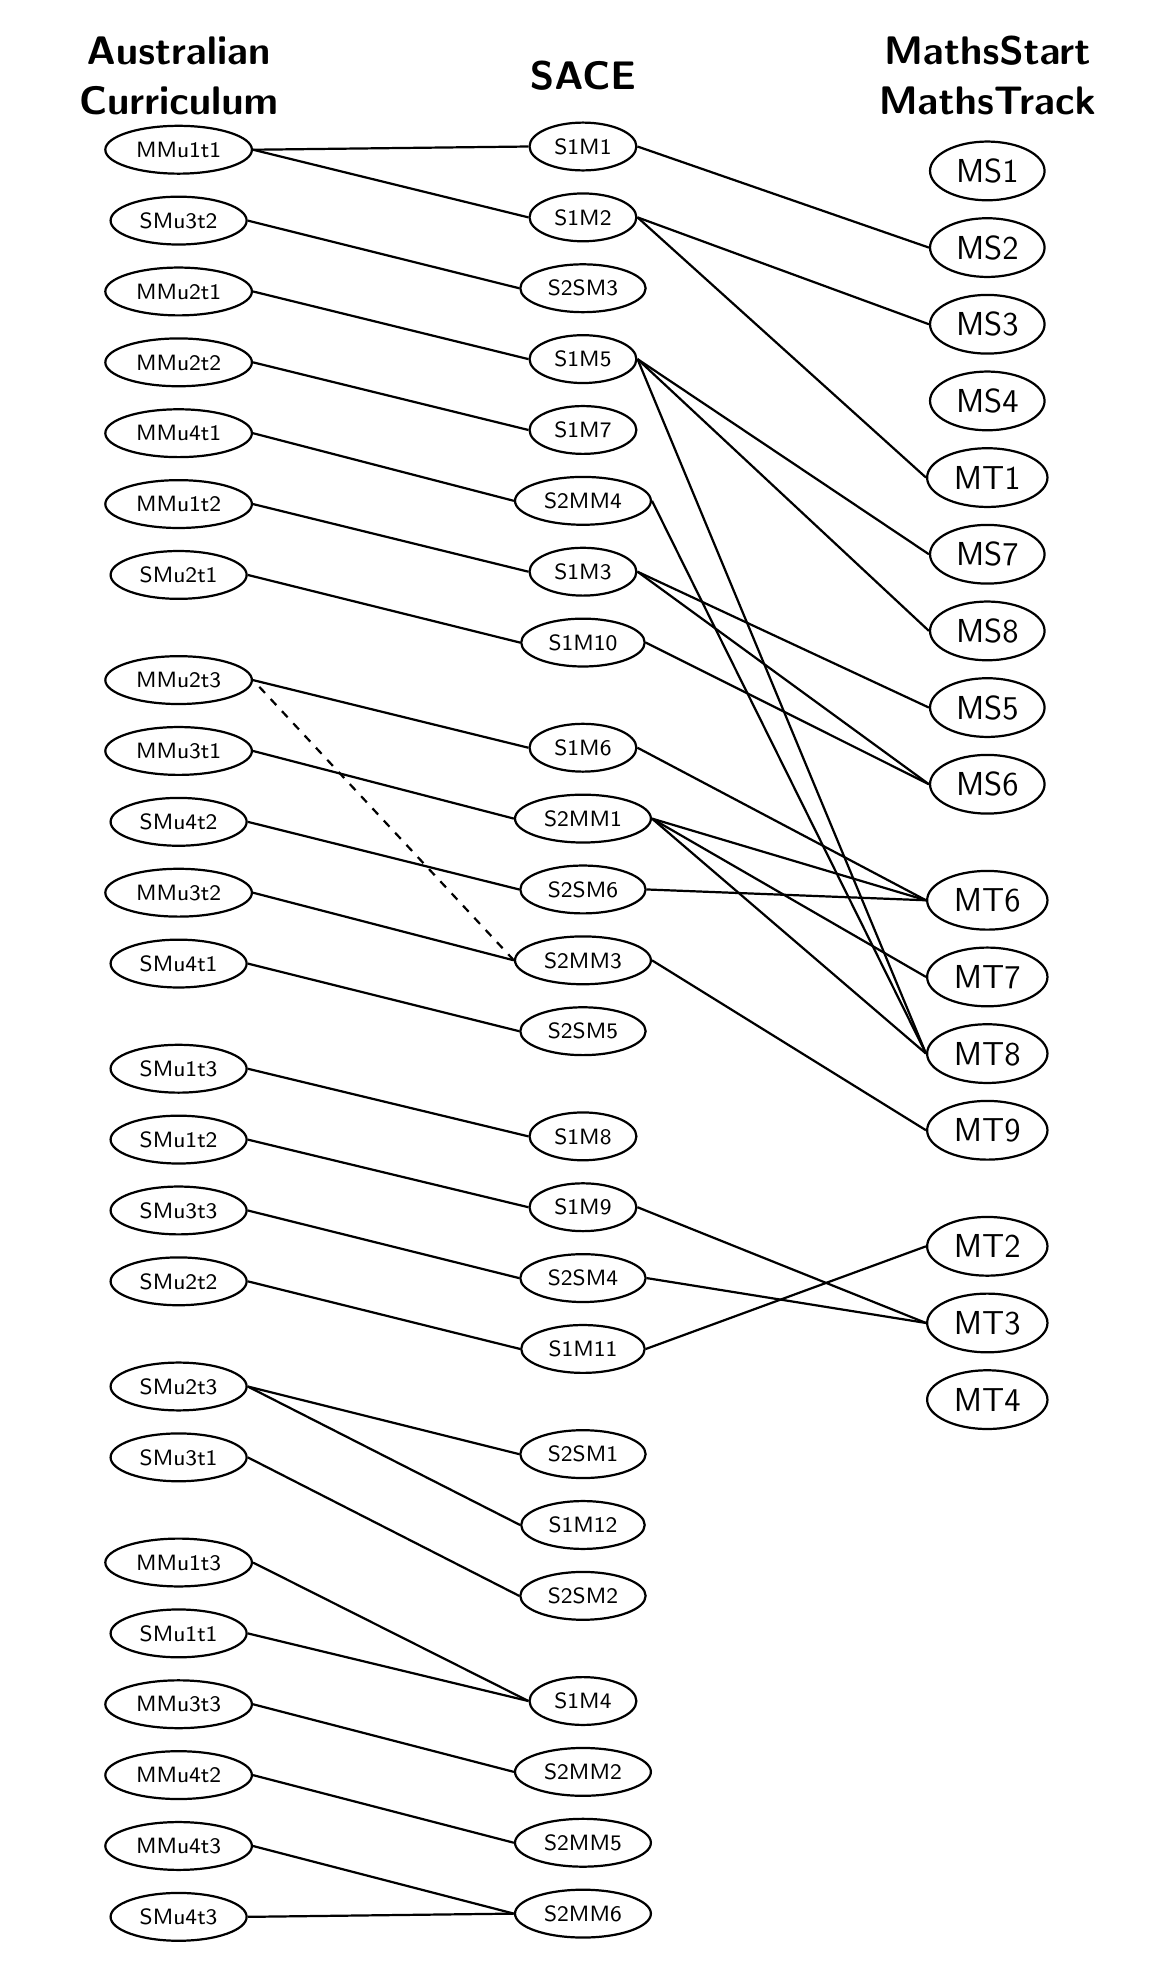
\begin{tikzpicture}[node distance=0.9cm,thick,topic node/.style={ellipse,draw,font=\footnotesize},unit node/.style={ellipse,draw,font=\large}]

	% MathsStart and MathsTrack
	\node[font=\Large\bfseries, text width = 3.6cm, align=center] (ms) {MathsStart MathsTrack};
	% Functions and Graphs
  	\node[unit node] (ms1) [below=0.2cm of ms] {MS1};
  	\node[unit node] (ms2) [below=0.2cm of ms1] {MS2};
  	\node[unit node] (ms3) [below=0.2cm of ms2] {MS3};
  	\node[unit node] (ms4) [below=0.2cm of ms3] {MS4};
  	\node[unit node] (mt1) [below=0.2cm of ms4] {MT1};
  	\node[unit node] (ms7) [below=0.2cm of mt1] {MS7};
  	\node[unit node] (ms8) [below=0.2cm of ms7] {MS8};
  	\node[unit node] (ms5) [below=0.2cm of ms8] {MS5};
  	\node[unit node] (ms6) [below=0.2cm of ms5] {MS6};
	% Calculus
  	\node[unit node] (mt6) [below=0.7cm of ms6] {MT6};
  	\node[unit node] (mt7) [below=0.2cm of mt6] {MT7};
  	\node[unit node] (mt8) [below=0.2cm of mt7] {MT8};
  	\node[unit node] (mt9) [below=0.2cm of mt8] {MT9};
	% Geometry and Linear Algebra	
  	\node[unit node] (mt2) [below=0.7cm of mt9] {MT2};
  	\node[unit node] (mt3) [below=0.2cm of mt2] {MT3};
  	\node[unit node] (mt4) [below=0.2cm of mt3] {MT4};
  	
	% SACE
	\node[font=\Large\bfseries] (sace) [left=2.4cm of ms] {SACE};
	% Functions and Graphs
  	\node[topic node] (ss1m1) [below of=sace] {S1M1};
  	\node[topic node] (ss1m2) [below of=ss1m1] {S1M2};
  	\node[topic node] (ss2sm3) [below of=ss1m2] {S2SM3};
  	\node[topic node] (ss1m5) [below of=ss2sm3] {S1M5};
  	\node[topic node] (ss1m7) [below of=ss1m5] {S1M7};
  	\node[topic node] (ss2mm4) [below of=ss1m7] {S2MM4};
  	\node[topic node] (ss1m3) [below of=ss2mm4] {S1M3};
  	\node[topic node] (ss1m10) [below of=ss1m3] {S1M10};
	% Calculus
  	\node[topic node] (ss1m6) [below=0.7cm of ss1m10] {S1M6};
  	\node[topic node] (ss2mm1) [below of=ss1m6] {S2MM1};
  	\node[topic node] (ss2sm6) [below of=ss2mm1] {S2SM6};  	
  	\node[topic node] (ss2mm3) [below of=ss2sm6] {S2MM3};
  	\node[topic node] (ss2sm5) [below of=ss2mm3] {S2SM5};
	% Geometry and Linear Algebra
  	\node[topic node] (ss1m8) [below=0.7cm of ss2sm5] {S1M8};
	\node[topic node] (ss1m9) [below of=ss1m8] {S1M9};
  	\node[topic node] (ss2sm4) [below of=ss1m9] {S2SM4};
  	\node[topic node] (ss1m11) [below of=ss2sm4] {S1M11};
  	% Complex Numbers
  	\node[topic node] (ss2sm1) [below=0.7cm of ss1m11] {S2SM1};
  	\node[topic node] (ss1m12) [below of=ss2sm1] {S1M12};
  	\node[topic node] (ss2sm2) [below of=ss1m12] {S2SM2};
	% Probability and Statistics	
  	\node[topic node] (ss1m4) [below=0.7cm of ss2sm2] {S1M4};
  	\node[topic node] (ss2mm2) [below of=ss1m4] {S2MM2}; 	
  	\node[topic node] (ss2mm5) [below of=ss2mm2] {S2MM5};
  	\node[topic node] (ss2mm6) [below of=ss2mm5] {S2MM6};
  	
  	
	% Australian Curriculum
	\node[font=\Large\bfseries, text width = 3.6cm, align=center] (ac) [left=2.4cm of sace] {Australian Curriculum};
	% Functions and Graphs
  	\node[topic node] (acmmmu1t1) [below=0cm of ac] {MMu1t1};
  	\node[topic node] (acmsmu3t2) [below of=acmmmu1t1] {SMu3t2};
  	\node[topic node] (acmmmu2t1) [below of=acmsmu3t2] {MMu2t1};
  	\node[topic node] (acmmmu2t2) [below of=acmmmu2t1] {MMu2t2};
  	\node[topic node] (acmmmu4t1) [below of=acmmmu2t2] {MMu4t1};
  	\node[topic node] (acmmmu1t2) [below of=acmmmu4t1] {MMu1t2};
  	\node[topic node] (acmsmu2t1) [below of=acmmmu1t2] {SMu2t1};
	% Calculus
  	\node[topic node] (acmmmu2t3) [below=0.7cm of acmsmu2t1] {MMu2t3};
  	\node[topic node] (acmmmu3t1) [below of=acmmmu2t3] {MMu3t1};
  	\node[topic node] (acmsmu4t2) [below of=acmmmu3t1] {SMu4t2};
  	\node[topic node] (acmmmu3t2) [below of=acmsmu4t2] {MMu3t2};
  	\node[topic node] (acmsmu4t1) [below of=acmmmu3t2] {SMu4t1};
	% Geometry and Linear Algebra
  	\node[topic node] (acmsmu1t3) [below=0.7cm of acmsmu4t1] {SMu1t3};
  	\node[topic node] (acmsmu1t2) [below of=acmsmu1t3] {SMu1t2};
  	\node[topic node] (acmsmu3t3) [below of=acmsmu1t2] {SMu3t3};
  	\node[topic node] (acmsmu2t2) [below of=acmsmu3t3] {SMu2t2};
	% Complex Numbers
  	\node[topic node] (acmsmu2t3) [below=0.7cm of acmsmu2t2] {SMu2t3};
  	\node[topic node] (acmsmu3t1) [below of=acmsmu2t3] {SMu3t1};
	% Probability and Statistics
  	\node[topic node] (acmmmu1t3) [below=0.7cm of acmsmu3t1] {MMu1t3};
  	\node[topic node] (acmsmu1t1) [below of=acmmmu1t3] {SMu1t1};
  	\node[topic node] (acmmmu3t3) [below of=acmsmu1t1] {MMu3t3};
  	\node[topic node] (acmmmu4t2) [below of=acmmmu3t3] {MMu4t2};
  	\node[topic node] (acmmmu4t3) [below of=acmmmu4t2] {MMu4t3};
  	\node[topic node] (acmsmu4t3) [below of=acmmmu4t3] {SMu4t3};

	% Australian Curriculum -- SACE links
	\draw (ss1m1.west) -- (acmmmu1t1.east);
	\draw (ss1m2.west) -- (acmmmu1t1.east);
	\draw (ss1m3.west) -- (acmmmu1t2.east);
	\draw (ss1m4.west) -- (acmmmu1t3.east);
	\draw (ss1m4.west) -- (acmsmu1t1.east);
	\draw (ss1m5.west) -- (acmmmu2t1.east);
	\draw (ss1m6.west) -- (acmmmu2t3.east);
	\draw (ss1m7.west) -- (acmmmu2t2.east);
	\draw (ss1m8.west) -- (acmsmu1t3.east);
	\draw (ss1m9.west) -- (acmsmu1t2.east);
	\draw (ss1m10.west) -- (acmsmu2t1.east);
	\draw (ss1m11.west) -- (acmsmu2t2.east);
	\draw (ss1m12.west) -- (acmsmu2t3.east);
		
	\draw (ss2mm1.west) -- (acmmmu3t1.east);
	\draw (ss2mm2.west) -- (acmmmu3t3.east);
	\draw (ss2mm3.west) -- (acmmmu3t2.east);
	\draw[dashed] (ss2mm3.west) -- (acmmmu2t3.east);
	\draw (ss2mm4.west) -- (acmmmu4t1.east);
	\draw (ss2mm5.west) -- (acmmmu4t2.east);
	\draw (ss2mm6.west) -- (acmmmu4t3.east);
	\draw (ss2mm6.west) -- (acmsmu4t3.east);

	\draw (ss2sm1.west) -- (acmsmu2t3.east);
	\draw (ss2sm2.west) -- (acmsmu3t1.east);
	\draw (ss2sm3.west) -- (acmsmu3t2.east);
	\draw (ss2sm4.west) -- (acmsmu3t3.east);
	\draw (ss2sm5.west) -- (acmsmu4t1.east);
	\draw (ss2sm6.west) -- (acmsmu4t2.east);

	% MathsTrack to SACE links
	\draw (mt1.west) -- (ss1m2.east);
	\draw (mt2.west) -- (ss1m11.east);
	\draw (mt3.west) -- (ss1m9.east);
	\draw (mt3.west) -- (ss2sm4.east);
	\draw (mt6.west) -- (ss1m6.east);
	\draw (mt6.west) -- (ss2mm1.east);
	\draw (mt6.west) -- (ss2sm6.east);
	\draw (mt7.west) -- (ss2mm1.east);
	\draw (mt8.west) -- (ss1m5.east);
	\draw (mt8.west) -- (ss2mm1.east);
	\draw (mt8.west) -- (ss2mm4.east);
	\draw (mt9.west) -- (ss2mm3.east);

	% MathsTrack to SACE links
	\draw (ms2.west) -- (ss1m1.east);
	\draw (ms3.west) -- (ss1m2.east);
	\draw (ms5.west) -- (ss1m3.east);
	\draw (ms6.west) -- (ss1m3.east);
	\draw (ms6.west) -- (ss1m10.east);
	\draw (ms7.west) -- (ss1m5.east);
	\draw (ms8.west) -- (ss1m5.east);


  	
\end{tikzpicture}
\end{document}
\caption{Curriculum Mapping\label{fig:mappingByTopic}}
\end{center}
\end{figure}



\subsection{\gls{ac} and \gls{sace} to MathsStart and MathsTrack}

In the broad sense of areas of mathematics the topcs can be grouped into naturally, as discussed above in \refsec{content}, the topics that are covered in the \gls{ac} and \gls{sace} but not in MathsStart or MathsTrack are complex numbers, and Probability/ Statistics/ Combinatorics. So given that those areas are not covered in MathsStart or MathsTrack at all, lets take a look in more detail (at a key concept level) at the alignment of the topics that are covered in MathsStart and MathsTrack.

\begin{itemize}
	\item Functions and Graphs
	\item Calculus
	\item Geometry and Linear Algebra
\end{itemize}





MS4: Note the link to S2SM3 

\begin{itemize}
	\item MS1: Maybe Introduce Interval Notation along with Intervals?
	\item MT2: Gauss-Jordan is used to introduce the concept of a Matrix Inverse, altough very relevant to first year maths, not in the AC/ SACE at all.
	\item MT6: Note that the concept of the normal to a curve is introduced, but is not in any curriculum (or first year maths course that I know of?)
	\item MT8: There are many ways to introduce $e = 2.718\hdots$, but the way it is introduced in MathsTrack is (perhaps coincidentally), precisely the same as the way it is introduced in SACE (and AC?).
	\item MT8: Surge Models are introduced which are not used anywhere else.
	\item MT8: Logistic Models are introduced, but not as a DE just as a model.
	\item MT9: Looks at area between two curves, a concept covered in \gls{sace} in 
\end{itemize}

My reccomendations for MathsStart would be to include some work on fractions, index laws, and more emphasise on re-arranging equations  as in my experience these are the topics and concepts that students need the most from middle school mathematics (up to year 10) and form foundations for building other concepts with in senior highschool. 



\cleardoublepage
\chapter{Moving Forward: Improvements} 
\label{chap:recommendations}

\lipsum[1]

\section{Current Strengths of MathsStart and MathsTrack}

Moving foward is a two-part process:
\begin{itemize}
	\item Recognise what is being done well, encourage and recognise it, and continue to support its ongoing excellence.
	\item Recognise what can be improved on, gaps that may exist, and address them with specific actionable changes.
\end{itemize}

\subsection{SQWIGLES}

See \href{https://blogs.adelaide.edu.au/maths-learning/2016/09/20/sqwigles/}{David Butler's blog post about it}

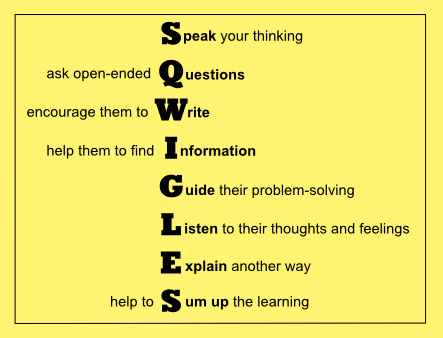
\includegraphics{./files/sqwigles.png}



\subsection{Staff Culture at the Maths Learning Center}

\subsection{Self-Paced Assessment and Content Speed (!!!)}

Link to Maths Anxiety literature review.



\cleardoublepage
\chapter*{Conclusions and Reccomendations}
\addcontentsline{toc}{chapter}{Conclusions and Reccomendations}

With respect to the bridging courses run through the university of adelaide's maths learning centre: MathsStart and MathsTrack,
\begin{itemize}
	\item The self-paced and feedback focused approach to assessment is certainly the highlight of the programs, should be continued, encouraged, potentially further resourced, expanded, and reccomended to other bridging course facilitators.
	\item The role of bridging courses as what is often student's first experience at university implies that potentially students wellbeing and retention could be improved by structuring the programs to provide more opportunities for students to meet each other and work together: either in the maths learning center drop-in area, or a seperate area, but potentially assigning a certain time on a certain day perhaps weekly or fortnightly during which students are encouraged to come and work together, could allow them to make freinds, build social networks, and better aclimitise them to the university environment in order to better prepare them for success in their studies.
	\item The smallest but perhaps easiest to implement improvement could be to better align the course content with curriculum, both the highschool curriculum (\gls{ac}/ \gls{sace}) in the case of students doing the bridging course to then comence study interstate or overseas, or with specific first year entry level courses, to better match the potential gaps in knowledge students may encounter.
\end{itemize}

% Bibliography/ References
\glsresetall
\bibliographystyle{apacite}
\bibliography{citations} 

\end{document}


